\section{Training and Architecture}

%%%%%%%%%%%%%%%%%%%%%%%%%%%%%%%%%%%%%%%%%%%%%%%%%%
\begin{frame}[fragile]{Which Network!}


		\begin{itemize}
			\item[--] \textbf{Pattern}: is a sequence of characters.
			\item  Unlike feedforward neural networks, RNNs can use their internal state (memory) to process sequences of inputs.
			\item In theory, RNNs are capable of handling long-term dependencies. 	However, in practice they do not, due to the \alert{exploding gradient problem}
			\item LSTMs was designed to solve the long-term dependency problem using internal memory gates.
		\end{itemize}
		
\end{frame}
%%%%%%%%%%%%%%%%%%%%%%%%%%%%%%%%%%%%%%%%%%%%%%%%%%
\begin{frame}[fragile]{RNN, Architectures}
\begin{figure}[t]
	\minipage{\textwidth}
	\centering
	\begin{tikzpicture}[scale=2]

% The grid
%  \draw[step=0.5, gray!40, very thin] (-1,-1) grid (8,8);

% LSTM frame
\def \yONE {0.75}

\def \sigmoidWidth  {0.5}
\def \sigmoidInDist {0.2}
\def \sigmoidHeight  {0.5}
\def \yB  {1.5}
\def \yD  {2.75}
\def \xZERO  {0}
\def \xONE  {2}
\def \xTWO  {3.5}
\def \xTHREE  {5}
\def \xFOUR  {7}
\def \shift {1}
\def \bigR {0.25cm}
%%%%%%%%%%%%%%%%%%%%%first one 
% First Sigmoid
\draw[fill=LightYellow] (\xONE, \yB) rectangle (\xONE+ \sigmoidWidth, \yB + \sigmoidHeight) node[pos=0.5] {\Large$\sigma$};
% Upper Arrow Sigmoid 
\draw[arrows=-latex, line width=2.5pt]  (\xONE + \sigmoidWidth/2, \yB +\sigmoidHeight) -- (\xONE + \sigmoidWidth/2, 2.6);
% Circle X_{t+1}
\draw[thick,fill=LightBlue1] (\xONE + \sigmoidWidth/2, \yONE ) circle (\bigR) node {\Large$x_0$};
% Down Arrow X_{t+1}
\draw[arrows=-latex,line width=2.5pt] (\xONE + \sigmoidWidth/2, \yONE + 0.25)  --  (\xONE + \sigmoidWidth/2, \yB);
% Circle H{t} 
\draw[thick,fill=LightPurple1] (\xONE + \sigmoidWidth/2, \yD) circle (\bigR) node {\Large$h_0$};
% Right Arrow H{t} 
\draw[arrows=-latex, line width=2.5pt] (\xONE + \sigmoidWidth/2+\sigmoidWidth/2, 1.75)   
--  (\xTWO, 1.75)
node[right, xshift=-0.9cm, yshift=0.4cm,] {\Large$h_0$};
%%%%%%%%%%%%%%%%%%%%%second one 
% First Sigmoid
%%%%%%%%%%%%%%%%%%%%%first one 
% First Sigmoid
\draw[fill=LightYellow] (\xTWO, \yB) rectangle (\xTWO+ \sigmoidWidth, \yB + \sigmoidHeight) node[pos=0.5] {\Large$\sigma$};
% Upper Arrow Sigmoid 
\draw[arrows=-latex, line width=2.5pt]  (\xTWO + \sigmoidWidth/2, \yB +\sigmoidHeight) -- (\xTWO + \sigmoidWidth/2, 2.6);
% Circle X_{t+1}
\draw[thick,fill=LightBlue1] (\xTWO + \sigmoidWidth/2, \yONE ) circle (\bigR) node {\Large$x_1$};
% Down Arrow X_{t+1}
\draw[arrows=-latex,line width=2.5pt] (\xTWO + \sigmoidWidth/2, \yONE + 0.25)  --  (\xTWO + \sigmoidWidth/2, \yB);
% Circle H{t} 
\draw[thick,fill=LightPurple1] (\xTWO + \sigmoidWidth/2, \yD) circle (\bigR) node {\Large$h_1$};
% Right Arrow H{t} 
\draw[arrows=-latex, line width=2.5pt] (\xTWO + \sigmoidWidth/2+\sigmoidWidth/2, 1.75)   
--  (\xTHREE, 1.75)
node[right, xshift=-0.9cm, yshift=0.4cm,] {\Large$h_1$};

%%%%%%%%%%%%%%%%%%%%%first one 
% First Sigmoid
\draw[fill=LightYellow] (\xTHREE, \yB) rectangle (\xTHREE+ \sigmoidWidth, \yB + \sigmoidHeight) node[pos=0.5] {\Large$\sigma$};
% Upper Arrow Sigmoid 
\draw[arrows=-latex, line width=2.5pt]  (\xTHREE + \sigmoidWidth/2, \yB +\sigmoidHeight) -- (\xTHREE + \sigmoidWidth/2, 2.6);
% Circle X_{t+1}
\draw[thick,fill=LightBlue1] (\xTHREE + \sigmoidWidth/2, \yONE ) circle (\bigR) node {\Large$x_2$};
% Down Arrow X_{t+1}
\draw[arrows=-latex,line width=2.5pt] (\xTHREE + \sigmoidWidth/2, \yONE + 0.25)  --  (\xTHREE + \sigmoidWidth/2, \yB);
% Circle H{t} 
\draw[thick,fill=LightPurple1] (\xTHREE + \sigmoidWidth/2, \yD) circle (\bigR) node {\Large$h_2$};
% Right Arrow H{t} 
\draw[arrows=-latex, line width=2.5pt] (\xTHREE + \sigmoidWidth/2+\sigmoidWidth/2, 1.75)   
--  (\xFOUR, 1.75)
node[right, xshift=-0.9cm, yshift=0.4cm,] {\Large$h_2$};

%%%%%%%%%%%%%%%%%%%%%first one 
% First Sigmoid
\draw[fill=LightYellow] (\xFOUR, \yB) rectangle (\xFOUR+ \sigmoidWidth, \yB + \sigmoidHeight) node[pos=0.5] {\Large$\sigma$};
% Upper Arrow Sigmoid 
\draw[arrows=-latex, line width=2.5pt]  (\xFOUR + \sigmoidWidth/2, \yB +\sigmoidHeight) -- (\xFOUR + \sigmoidWidth/2, 2.6);
% Circle X_{t+1}
\draw[thick,fill=LightBlue1] (\xFOUR + \sigmoidWidth/2, \yONE ) circle (\bigR) node {\Large$x_{t}$};
% Down Arrow X_{t+1}
\draw[arrows=-latex,line width=2.5pt] (\xFOUR + \sigmoidWidth/2, \yONE + 0.25)  --  (\xFOUR + \sigmoidWidth/2, \yB);
% Circle H{t} 
\draw[thick,fill=LightPurple1] (\xFOUR + \sigmoidWidth/2, \yD) circle (\bigR) node {\Large$h_t$};
% Right Arrow H{t} 
\draw[arrows=-latex, line width=2.5pt] (\xFOUR + \sigmoidWidth/2+\sigmoidWidth/2, 1.75)   
--  (\xFOUR + \sigmoidWidth + \sigmoidWidth, 1.75)
node[right, xshift=-0.9cm, yshift=0.4cm,] {\Large$h_t$};
\node[text width=1cm] at (\xFOUR-.75,1) 
{\LARGE....};

%%%%%%%%%%%%%%%%%%%%%first one 
% First Sigmoid
\draw[fill=LightYellow] (\xZERO, \yB) rectangle (\xZERO+ \sigmoidWidth, \yB + \sigmoidHeight) node[pos=0.5] {\Large$\sigma$};
% Upper Arrow Sigmoid 
\draw[arrows=-latex, line width=2.5pt]  (\xZERO + \sigmoidWidth/2, \yB +\sigmoidHeight) -- (\xZERO + \sigmoidWidth/2, 2.6);
% Circle X_{t+1}
\draw[thick,fill=LightBlue1] (\xZERO + \sigmoidWidth/2, \yONE ) circle (\bigR) node {\Large$x_0$};
% Down Arrow X_{t+1}
\draw[arrows=-latex,line width=2.5pt] (\xZERO + \sigmoidWidth/2, \yONE + 0.25)  --  (\xZERO + \sigmoidWidth/2, \yB);
% Circle H{t} 
\draw[thick,fill=LightPurple1] (\xZERO + \sigmoidWidth/2, \yD) circle (\bigR) node {\Large$h_0$};
% Right Arrow H{t} 
\draw[line width=2.5pt] (\xZERO + \sigmoidWidth/2+\sigmoidWidth/2, 1.75)   
--  (.5+\sigmoidWidth/2, 1.75);

\draw[line width=2.5pt] (.5+\sigmoidWidth/2, 1.73)   
--  (.5+\sigmoidWidth/2, 2.25);

\draw[line width=2.5pt] (.5+\sigmoidWidth/2, 2.23)   
--  (\xZERO + \sigmoidWidth/2+.03, 2.23);

\draw[line width=2.5pt] (\xZERO + \sigmoidWidth/2-.03, 2.23)   
--  (\xZERO - \sigmoidWidth/2, 2.23);

\draw[line width=2.5pt] (\xZERO - \sigmoidWidth/2, 2.25)
--  (\xZERO - \sigmoidWidth/2, 1.75);

\draw[arrows=-latex,line width=2.5pt] (\xZERO-.02 - \sigmoidWidth/2, 1.75)
--  (\xZERO , 1.75);

\node[text width=1cm] at (1.5,1.75) {\LARGE=};
\end{tikzpicture}

	\endminipage\hfill
	\caption{Recurrent Neural Networks Loops adapted from~\cite{colah}}\label{Fig:RNN_Rolled_Loop}
	
\end{figure}%
\end{frame}

%%%%%%%%%%%%%%%%%%%%%%%%%%%%%%%%%%%%%%%%%%%%%%%%%%
\begin{frame}[fragile]{RNN, Architectures}
\begin{figure}[t]
	\minipage{0.3\textwidth}
	\begin{tikzpicture}[scale=1.45]


% The grid
% \draw[step=0.5, gray!40, very thin] (0,0) grid (8,4);

% LSTM frame
\def \yONE {0.5}
\def \yTWO {3.3}
\draw[rounded corners=10pt, very thick, fill=LightGreen]  (1.5, 0.5) rectangle (5, 2.3);

\def \sigmoidWidth  {0.45}
\def \sigmoidInDist {0.2}
\def \sigmoidHeight  {0.3}
\def \yB  {1.3}
\def \yD  {2}
\def \shift {0.3}
\def \bigR {0.25cm}
\def \C    {1}
\def \xBigCicleONE {2}
\def \xBigCicleTWO {5.5 + 0.25}
\def \levelB {1}

% Second times operator and add operator
\def \xTimesB {2.6}
\def \yC      {1}
\def \xOfThirdSigmoid {\xSSS + \sigmoidWidth/2}


% Square tanh
\draw[fill=LightYellow]  (3,1.5-\sigmoidHeight/2) 
rectangle 
(3 +\sigmoidWidth, 1.5-\sigmoidHeight/2 +\sigmoidHeight)
node[pos=0.5] {\scriptsize\textit{tanh}};

%tanh upper line
\draw[line width=2.5pt,gray]  (3.2,1.65) -- (3.2, \yD);


%line A upper left input from previous cell
%\draw[arrows=-latex,line width=2.5pt,gray]  (1, \yD) -- (1.5, \yD);

%line A upper left input after cell
\draw[line width=2.5pt,gray]  (1.5, \yD) -- (2.4, \yD);

\draw[arrows=-latex, line width=2.5pt,gray] (2.39, \yD)  to[out=270, in=180] (3,1.5);

%line A upper from tanh to rictangle border
\draw[line width=2.5pt,gray]  (3.2, \yD) -- (5, \yD);

%line A upper from rictangle border to next cell
\draw[arrows=-latex,line width=2.5pt]  (5, \yD) -- (5.5, \yD);


%level B line 
\draw[line width=2.5pt,gray] (2.2, \levelB) 
--
(2.4, \levelB);

%second line last angle connected to sigmoid 

\draw[arrows=-latex, line width=2.5pt,gray] (2.39,1) 
to[out=90, in=180] 
(3,1.5);



\draw[thick,fill=LightBlue] (\xBigCicleONE, \yONE+.4 - \C) circle (\bigR) node {$x_{t-1}$};

% x_t line
\draw[line width=2.5pt,gray] (\xBigCicleONE, \yONE -\C +0.65) 
--
(\xBigCicleONE, \yONE -\C +0.25 + 1.1);

\draw[line width=2.5pt,gray] (\xBigCicleONE, \yONE -\C +0.25 + 1.1)
to[out=90, in=180]
(2.25, 1);


\draw[thick,fill=LightPurple] (\xBigCicleTWO-1, \yTWO -1.15 + \C) circle (\bigR) node {$h_{t-1}$};
%h_T lines
\draw[arrows=-latex, line width=2.5pt,gray]
(\xBigCicleTWO-1, \yD )
--
(\xBigCicleTWO-1, \yTWO -1.4 + \C);


\end{tikzpicture}

	\endminipage\hfill
	\minipage{0.3\textwidth}
	\begin{tikzpicture}[scale=1.45]


% The grid
% \draw[step=0.5, gray!40, very thin] (0,0) grid (8,4);

% LSTM frame
\def \yONE {0.5}
\def \yTWO {3.3}
\draw[rounded corners=10pt, very thick, fill=LightGreen]  (1.5, 0.5) rectangle (5, 2.3);

\def \sigmoidWidth  {0.45}
\def \sigmoidInDist {0.2}
\def \sigmoidHeight  {0.3}
\def \yB  {1.3}
\def \yD  {2}
\def \shift {0.3}

% Square tanh
\draw[fill=LightYellow]  (3,1.5-\sigmoidHeight/2) 
rectangle 
(3 +\sigmoidWidth, 1.5-\sigmoidHeight/2 +\sigmoidHeight)
node[pos=0.5] {\scriptsize\textit{tanh}};

%tanh upper line
\draw[line width=2.5pt]  (3.2,1.65) -- (3.2, \yD);

% Second times operator and add operator
\def \xTimesB {2.6}
\def \yC      {1}

%line A upper left input from previous cell
%\draw[arrows=-latex,line width=2.5pt]  (1, \yD) -- (1.5, \yD);

%line A upper left input after cell
\draw[line width=2.5pt]  (1.5, \yD) -- (2.4, \yD);

\draw[arrows=-latex, line width=2.5pt] (2.39, \yD)  to[out=270, in=180] (3,1.5);

%line A upper from tanh to rictangle border
\draw[line width=2.5pt]  (3.2, \yD) -- (5, \yD);

%line A upper from rictangle border to next cell
\draw[arrows=-latex,line width=2.5pt]  (5, \yD) -- (5.5, \yD);


\def \levelB {1}
%level B line 
\draw[line width=2.5pt] (2.2, \levelB) 
--
(2.4, \levelB);

\def \xOfThirdSigmoid {\xSSS + \sigmoidWidth/2}
%second line last angle connected to sigmoid 

\draw[arrows=-latex, line width=2.5pt] (2.39,1) 
to[out=90, in=180] 
(3,1.5);


\def \bigR {0.25cm}
\def \bigRTWO {0.4cm}
\def \C    {1}
\def \xBigCicleONE {2}
\def \xBigCicleTWO {5.5 + 0.25}

\draw[thick,fill=LightBlue] (\xBigCicleONE, \yONE+.4 - \C) circle (\bigR) node {$x_{t}$};

% x_t line
\draw[line width=2.5pt] (\xBigCicleONE, \yONE -\C +0.65) 
--
(\xBigCicleONE, \yONE -\C +0.25 + 1.1);

\draw[line width=2.5pt] (\xBigCicleONE, \yONE -\C +0.25 + 1.1)
to[out=90, in=180]
(2.25, 1);



\draw[thick,fill=LightPurple] (\xBigCicleTWO-1, \yTWO -1.15 + \C) circle (\bigR) node {$h_{t}$};
%h_T lines
\draw[arrows=-latex, line width=2.5pt]
(\xBigCicleTWO-1, \yD )
--
(\xBigCicleTWO-1, \yTWO -1.4 + \C);


\end{tikzpicture}

	\endminipage\hfill
	\minipage{0.3\textwidth}%
	\begin{tikzpicture}[scale=1.45]


% The grid
% \draw[step=0.5, gray!40, very thin] (0,0) grid (8,4);

% LSTM frame
\def \yONE {0.5}
\def \yTWO {3.3}
\draw[rounded corners=10pt, very thick, fill=LightGreen]  (1.5, 0.5) rectangle (5, 2.3);

\def \sigmoidWidth  {0.45}
\def \sigmoidInDist {0.2}
\def \sigmoidHeight  {0.3}
\def \yB  {1.3}
\def \yD  {2}
\def \shift {0.3}
\def \bigRTWO {0.4cm}
% Square tanh
\draw[fill=LightYellow]  (3,1.5-\sigmoidHeight/2) 
rectangle 
(3 +\sigmoidWidth, 1.5-\sigmoidHeight/2 +\sigmoidHeight)
node[pos=0.5] {\scriptsize\textit{tanh}};

%tanh upper line
\draw[line width=2.5pt,gray]  (3.2,1.65) -- (3.2, \yD);

% Second times operator and add operator
\def \xTimesB {2.6}
\def \yC      {1}

%line A upper left input from previous cell
%\draw[arrows=-latex,line width=2.5pt]  (1, \yD) -- (1.5, \yD);

%line A upper left input after cell
\draw[line width=2.5pt,gray]  (1.5, \yD) -- (2.4, \yD);

\draw[arrows=-latex, line width=2.5pt,gray] (2.39, \yD)  to[out=270, in=180] (3,1.5);

%line A upper from tanh to rictangle border
\draw[line width=2.5pt,gray]  (3.2, \yD) -- (5, \yD);

%line A upper from rictangle border to next cell
\draw[arrows=-latex,line width=2.5pt]  (5, \yD) -- (5.6, \yD);


\def \levelB {1}
%level B line 
\draw[line width=2.5pt,gray] (2.2, \levelB) 
--
(2.4, \levelB);

\def \xOfThirdSigmoid {\xSSS + \sigmoidWidth/2}
%second line last angle connected to sigmoid 

\draw[arrows=-latex, line width=2.5pt,gray] (2.39,1) 
to[out=90, in=180] 
(3,1.5);


\def \bigR {0.25cm}
\def \C    {1}
\def \xBigCicleONE {2}
\def \xBigCicleTWO {5.5 + 0.25}

\draw[thick,fill=LightBlue] (\xBigCicleONE, \yONE+.4 - \C) circle (\bigR) node {$x_{t+1}$};

% x_t line
\draw[line width=2.5pt,gray] (\xBigCicleONE, \yONE -\C +0.65) 
--
(\xBigCicleONE, \yONE -\C +0.25 + 1.1);

\draw[line width=2.5pt,gray] (\xBigCicleONE, \yONE -\C +0.25 + 1.1)
to[out=90, in=180]
(2.25, 1);



\draw[thick,fill=LightPurple] (\xBigCicleTWO-1, \yTWO -1.15 + \C) circle (\bigR) node {$h_{t+1}$};
%h_T lines
\draw[arrows=-latex, line width=2.5pt,gray]
(\xBigCicleTWO-1, \yD )
--
(\xBigCicleTWO-1, \yTWO -1.4 + \C);


\end{tikzpicture}

	\endminipage
	\caption{A single recurrent layer adapted from~\cite{colah}}~\label{Fig:LSTM_SimpleRNN}
\end{figure}%
\end{frame}
%%%%%%%%%%%%%%%%%%%%%%%%%%%%%%%%%%%%%%%%%%%%%%%%%%

\begin{frame}[fragile]{LSTM Architectures}
\begin{center}
\begin{figure}[t]
	\minipage{0.8\textwidth}
	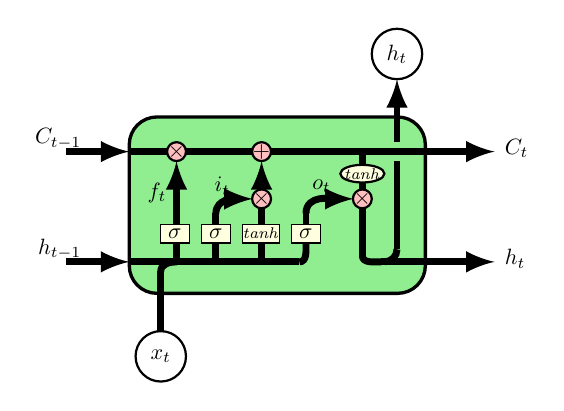
\begin{tikzpicture}[scale=.8, transform shape]

  % The grid
  % \draw[step=0.5, gray!40, very thin] (0,0) grid (8,4);

  % LSTM frame
  \def \yONE {0.5}
  \def \yTWO {3.3}
  \draw[rounded corners=10pt, very thick, fill=LightGreen]  (1.5, 0.5) rectangle (6.2, 3.3);

  \def \sigmoidWidth  {0.45}
  \def \sigmoidInDist {0.2}
  \def \sigmoidHeight  {0.3}
  \def \yB  {1.3}
  \def \yD  {2.75}
  \def \shift {0.3}
  % First Sigmoid
  \draw[fill=LightYellow] (2, \yB) rectangle (2+ \sigmoidWidth, \yB + \sigmoidHeight) node[pos=0.5] {$\sigma$};

  \def \r {.15cm}
  % The Upper times operator % first time from left
  \draw[thick, fill=pink] (2.25, \yD) circle (\r) node {$\times$};

  % Second Sigmoid
  \def \xS {2.45 +\sigmoidInDist}
  \draw[fill=LightYellow]  (\xS, \yB) rectangle (\xS +\sigmoidWidth, \yB + \sigmoidHeight) node[pos=0.5] {$\sigma$};

  % Square tanh
  \def \xSS {\xS +\sigmoidWidth + \sigmoidInDist}
  \draw[fill=LightYellow]  (\xSS, \yB) 
  rectangle 
  (\xSS +\sigmoidWidth +0.13, \yB +\sigmoidHeight)
  node[pos=0.5] {\scriptsize \textit{tanh}};

  % Third Sigoid
  \def \xSSS {\xSS +\sigmoidWidth +0.13 +\sigmoidInDist}
  \draw[fill=LightYellow]  (\xSSS, \yB) rectangle (\xSSS +\sigmoidWidth, \yB +\sigmoidHeight)
  node[pos=0.5] { $\sigma$};

  % Second times operator and add operator
  \def \xTimesB {3.6}
  \def \yC      {2}

  \draw[thick,fill=pink] (\xTimesB, \yC) circle (\r) node {$\times$};
  %%%%% first line sectond operator +
  \draw[thick, fill=pink] (\xTimesB, \yD) circle (\r) node {$+$};

  % Third times operator and its tanh
  \draw[thick,fill=pink] (\xTimesB +1.3 +\shift, \yC) circle (\r) node {$\times$};
  \draw[thick,fill=LightYellow] (\xTimesB +1.3 +\shift, \yC +.4)  
  ellipse (.35cm and .14cm) 
  node {\scriptsize \textit{tanh}};


  % LINES %%% Upper line from c_{t -1} till C_t
  \draw[arrows=-latex, line width=2.5pt]  (0.5, \yD) -- (1.5, \yD) node[left, xshift=-.6cm, yshift=0.2cm] {$C_{t-1}$};
  \draw[line width=2.5pt]  (1.5, \yD) -- (2.1, \yD);
  \draw[line width=2.5pt]  (2.4, \yD) -- (3.46, \yD);
  \draw[line width=2.5pt]  (3.75, \yD) -- (6.25 +0.2, \yD);

  \draw[arrows=-latex, line width=2.5pt]  (6.25, \yD) -- (7 + 0.3, \yD)
  node[right, xshift=0.0cm, yshift=0.05cm] {$C_t$};

  %%%%first line from left from sigmoid ft till times input from C_{t-1}
  \draw[arrows=-latex, line width=2.5pt]  (2.25, \yB +\sigmoidHeight) -- (2.25, 2.6)
  node[left, yshift=-0.5cm] {$f_t$};

  % Level B LINES
  \def \levelB {1}
   \draw[arrows=-latex, line width=2.5pt] (0.5, \levelB) -- (1.5, \levelB) node[left, xshift=-.6cm, yshift=0.2cm] {$h_{t-1}$};

  \draw[line width=2.5pt] (1.5, \levelB) 
  --
  (4.2, \levelB);

  \def \xOfThirdSigmoid {\xSSS + \sigmoidWidth/2}
  %second line last angle connected to sigmoid 
  \draw[line width=2.5pt] (4.2, \levelB) to[out=0,in=270] (\xOfThirdSigmoid, \yB);

  % Third Sigmoid up line
  % END (\xTimesB +1.3 - 0.19 , \yC)
  \draw[line width=2.5pt] (\xOfThirdSigmoid, \yB + \sigmoidHeight) 
  --
  (\xOfThirdSigmoid, \yB + \sigmoidHeight + 0.17) ;

  \draw[arrows=-latex, line width=2.5pt] (\xOfThirdSigmoid, \yB + \sigmoidHeight+0.17) 
  to[out=90, in=180] 
  (\xTimesB +1.3 -0.14 +\shift , \yC) 
  node [left, yshift=0.2cm, xshift=-0.2cm] {$o_t$};

  % tanh line
  \draw [line width=2.5pt] (\xTimesB, \levelB)
  --
  (\xTimesB, \yB);

  \draw [line width=2.5pt] (\xTimesB, \yB + \sigmoidHeight)
  --
  (\xTimesB, \yB + \sigmoidHeight +0.24);

  \draw [arrows=-latex, line width=2.5pt] (\xTimesB, 2.15)
  --
  (\xTimesB, 2.6);

  \draw[line width=2.5pt] (2.25, \levelB)
  --
  (2.25, \yB);
  
  \draw[line width=2.5pt] (\xS +\sigmoidWidth/2, \levelB)
  --
  (\xS +\sigmoidWidth/2, \yB);

  \draw[line width=2.5pt] (\xS +\sigmoidWidth/2, \yB +\sigmoidHeight)
  -- 
  (\xS +\sigmoidWidth/2, \yB +\sigmoidHeight + 0.17);

  \draw[arrows=-latex, line width=2.5pt] (\xS +\sigmoidWidth/2, \yB + \sigmoidHeight+0.17) 
  to[out=90, in=180] 
  (\xTimesB-0.14, \yC)
  node [left, yshift=0.2cm, xshift=-0.2cm] {$i_t$};

  \def \bigR {0.25cm}
  \def \bigRTWO {0.4cm}
  \def \C    {1}
  \def \xBigCicleONE {2}
  \def \xBigCicleTWO {5.5 + 0.25}
  \draw[thick] (\xBigCicleONE, \yONE - \C) circle (\bigRTWO) node {$x_{t}$};
  \draw[thick] (\xBigCicleTWO, \yTWO + \C) circle (\bigRTWO) node {$h_{t}$};

  % LINE Circle ONE
  \draw[line width=2.5pt] (\xBigCicleONE, \yONE -\C +0.4) 
  --
  (\xBigCicleONE, \yONE -\C +0.25 + 1.1);

  \draw[line width=2.5pt] (\xBigCicleONE, \yONE -\C +0.25 + 1.1)
  to[out=90, in=180]
  (2.25, 1);

  % LINE third \times
  \draw[line width=2.5pt] (\xTimesB +1.3 +\shift, 1.1)
  --
  (\xTimesB +1.3 +\shift, \yC - 0.15);

  \draw[line width=2.5pt] (5.5, 1) 
  --
  (6.25 +0.2, 1);
  
  \draw[arrows=-latex, line width=2.5pt] (6.25, 1) 
  --
  (7 + 0.3, 1)
  node[right, xshift=0.0cm, yshift=0.05cm,] {$h_t$};

%%% second line last angle connect the input with h_t output
  \draw[line width=2.5pt] (\xTimesB +1.3 +\shift, 1.1)
  to[out=270, in=180]
  (5.5, 1);


  \draw[line width=2.5pt] (\xTimesB +1.3 +\shift, 2.14)
  --
  (\xTimesB +1.3 +\shift, 2.26);


  \draw[line width=2.5pt] (\xTimesB +1.3 +\shift, \yD)
  --
  (\xTimesB +1.3 +\shift, 2.54);


  \draw[line width=2.5pt] (\xBigCicleTWO, \levelB +0.2)
  --
  (\xBigCicleTWO, 2.6);

%%%%% first horizontal line from the right angle connected to output ht
  \draw[line width=2.5pt] (\xBigCicleTWO - 0.2, \levelB)
  to[out=0, in=270]
  (\xBigCicleTWO, \levelB +0.2);


  \draw[arrows=-latex, line width=2.5pt]
  (\xBigCicleTWO, \yD +0.15)
  --
  (\xBigCicleTWO, 4-.1);

\end{tikzpicture}

	\endminipage
	\caption{LSTM internal cell adapted from~\cite{colah}}~\label{Fig:LSTM_Cell_Chaining}
\end{figure}%
\end{center}
\end{frame}
%%%%%%%%%%%%%%%%%%%%%%%%%%%%%%%%%%%%%%%%%%%%%%%%%%

\begin{frame}[fragile]{LSTM Architectures}
\begin{figure}[t]
	\minipage{0.32\textwidth}
	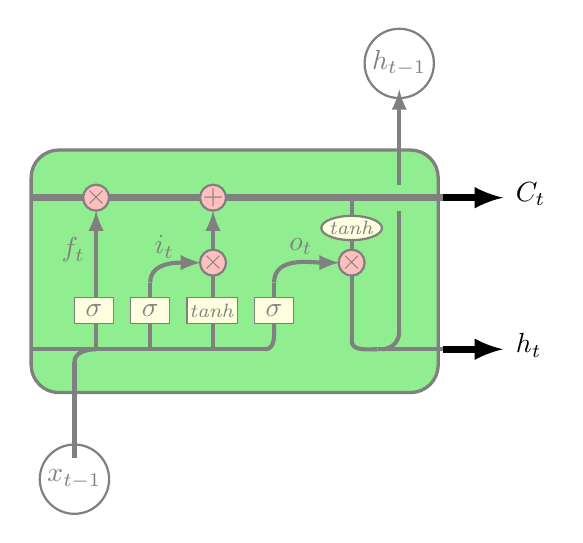
\begin{tikzpicture}[scale=1.1]

  % The grid
  % \draw[step=0.5, gray!40, very thin] (0,0) grid (8,4);

  % LSTM frame
  \def \yONE {0.5}
  \def \yTWO {3.3}
  \draw[rounded corners=10pt, very thick, gray,fill=LightGreen]  (1.5, 0.5) rectangle (6.2, 3.3);

  \def \sigmoidWidth  {0.45}
  \def \sigmoidInDist {0.2}
  \def \sigmoidHeight  {0.3}
  \def \yB  {1.3}
  \def \yD  {2.75}
  \def \shift {0.3}
  % First Sigmoid
  \draw[gray,fill=LightYellow] (2, \yB) rectangle (2+ \sigmoidWidth, \yB + \sigmoidHeight) node[pos=0.5] {$\sigma$};

  \def \r {.15cm}
  % The Upper times operator % first time from left
  \draw[thick, gray,fill=pink] (2.25, \yD) circle (\r) node {$\times$};

  % Second Sigmoid
  \def \xS {2.45 +\sigmoidInDist}
  \draw[gray,fill=LightYellow]  (\xS, \yB) rectangle (\xS +\sigmoidWidth, \yB + \sigmoidHeight) node[pos=0.5] {$\sigma$};

  % Square tanh
  \def \xSS {\xS +\sigmoidWidth + \sigmoidInDist}
  \draw[gray,fill=LightYellow]  (\xSS, \yB) 
  rectangle 
  (\xSS +\sigmoidWidth +0.13, \yB +\sigmoidHeight)
  node[pos=0.5] {\scriptsize \textit{tanh}};

  % Third Sigoid
  \def \xSSS {\xSS +\sigmoidWidth +0.13 +\sigmoidInDist}
  \draw[gray,fill=LightYellow]  (\xSSS, \yB) rectangle (\xSSS +\sigmoidWidth, \yB +\sigmoidHeight)
  node[pos=0.5] { $\sigma$};

  % Second times operator and add operator
  \def \xTimesB {3.6}
  \def \yC      {2}

  \draw[thick,gray,fill=pink] (\xTimesB, \yC) circle (\r) node {$\times$};
  %%%%% first line sectond operator +
  \draw[thick, gray,fill=pink] (\xTimesB, \yD) circle (\r) node {$+$};

  % Third times operator and its tanh
  \draw[thick,gray,fill=pink] (\xTimesB +1.3 +\shift, \yC) circle (\r) node {$\times$};
  \draw[thick,gray,fill=LightYellow] (\xTimesB +1.3 +\shift, \yC +.4)  
  ellipse (.35cm and .14cm) 
  node {\scriptsize \textit{tanh}};


  % LINES %%% Upper line from c_{t -1} till C_t
  %\draw[arrows=-latex, line width=2.5pt]  (0.85, \yD) -- (1.5, \yD) node[left, xshift=-.6cm, yshift=0.2cm] {$C_{t-1}$};
  \draw[line width=2.5pt, gray]  (1.5, \yD) -- (2.1, \yD);
  \draw[line width=2.5pt, gray]  (2.4, \yD) -- (3.46, \yD);
  \draw[line width=2.5pt,gray]  (3.75, \yD) -- (6.25 +0.2, \yD);

  \draw[arrows=-latex, line width=2.5pt]  (6.25, \yD) -- (6.75 +0.2, \yD)
  node[right, xshift=0.0cm, yshift=0.05cm] {$C_t$};

  %%%%first line from left from sigmoid ft till times input from C_{t-1}
  \draw[arrows=-latex, line width=1.5pt,gray]  (2.25, \yB +\sigmoidHeight) -- (2.25, 2.6)
  node[left, yshift=-0.5cm] {$f_t$};

  % Level B LINES
  \def \levelB {1}
  %\draw[arrows=-latex, line width=1.5pt,gray] (0.85, \levelB) -- (1.5, \levelB) node[left, xshift=-.6cm, yshift=0.2cm] {$h_{t-1}$};

  \draw[line width=1.5pt,gray] (1.5, \levelB) 
  --
  (4.2, \levelB);

  \def \xOfThirdSigmoid {\xSSS + \sigmoidWidth/2}
  %second line last angle connected to sigmoid 
  \draw[line width=1.5pt,gray] (4.2, \levelB) to[out=0,in=270] (\xOfThirdSigmoid, \yB);

  % Third Sigmoid up line
  % END (\xTimesB +1.3 - 0.19 , \yC)
  \draw[line width=1.5pt,gray] (\xOfThirdSigmoid, \yB + \sigmoidHeight) 
  --
  (\xOfThirdSigmoid, \yB + \sigmoidHeight + 0.17) ;

  \draw[arrows=-latex, line width=1.5pt,gray] (\xOfThirdSigmoid, \yB + \sigmoidHeight+0.17) 
  to[out=90, in=180] 
  (\xTimesB +1.3 -0.14 +\shift , \yC) 
  node [left, yshift=0.2cm, xshift=-0.2cm] {$o_t$};

  % tanh line
  \draw [line width=1.5pt,gray] (\xTimesB, \levelB)
  --
  (\xTimesB, \yB);

  \draw [line width=1.5pt,gray] (\xTimesB, \yB + \sigmoidHeight)
  --
  (\xTimesB, \yB + \sigmoidHeight +0.24);

  \draw [arrows=-latex, line width=1.5pt,gray] (\xTimesB, 2.15)
  --
  (\xTimesB, 2.6);

  \draw[line width=1.5pt,gray] (2.25, \levelB)
  --
  (2.25, \yB);
  
  \draw[line width=1.5pt,gray] (\xS +\sigmoidWidth/2, \levelB)
  --
  (\xS +\sigmoidWidth/2, \yB);

  \draw[line width=1.5pt,gray] (\xS +\sigmoidWidth/2, \yB +\sigmoidHeight)
  -- 
  (\xS +\sigmoidWidth/2, \yB +\sigmoidHeight + 0.17);

  \draw[arrows=-latex, line width=1.5pt,gray] (\xS +\sigmoidWidth/2, \yB + \sigmoidHeight+0.17) 
  to[out=90, in=180] 
  (\xTimesB-0.14, \yC)
  node [left, yshift=0.2cm, xshift=-0.2cm] {$i_t$};

  \def \bigR {0.25cm}
  \def \bigRTWO {0.4cm}
  \def \C    {1}
  \def \xBigCicleONE {2}
  \def \xBigCicleTWO {5.5 + 0.25}
  \draw[thick,gray] (\xBigCicleONE, \yONE - \C) circle (\bigRTWO) node {$x_{t-1}$};
  \draw[thick,gray] (\xBigCicleTWO, \yTWO + \C) circle (\bigRTWO) node {$h_{t-1}$};

  % LINE Circle ONE
  \draw[line width=1.5pt,gray] (\xBigCicleONE, \yONE -\C +0.25) 
  --
  (\xBigCicleONE, \yONE -\C +0.25 + 1.1);

  \draw[line width=1.5pt,gray] (\xBigCicleONE, \yONE -\C +0.25 + 1.1)
  to[out=90, in=180]
  (2.25, 1);

  % LINE third \times
  \draw[line width=1.5pt,gray] (\xTimesB +1.3 +\shift, 1.1)
  --
  (\xTimesB +1.3 +\shift, \yC - 0.15);

  \draw[line width=1.5pt,gray] (5.5, 1) 
  --
  (6.25 +0.2, 1);
  
  \draw[arrows=-latex,line width=2.5pt] (6.25, 1) 
  --
  (6.75 +0.2, 1)
  node[right, xshift=0.0cm, yshift=0.05cm,] {$h_t$};

%%% second line last angle connect the input with h_t output
  \draw[line width=1.5pt,gray] (\xTimesB +1.3 +\shift, 1.1)
  to[out=270, in=180]
  (5.5, 1);


  \draw[line width=1.5pt,gray] (\xTimesB +1.3 +\shift, 2.14)
  --
  (\xTimesB +1.3 +\shift, 2.26);


  \draw[line width=1.5pt,gray] (\xTimesB +1.3 +\shift, \yD)
  --
  (\xTimesB +1.3 +\shift, 2.54);


  \draw[line width=1.5pt,gray] (\xBigCicleTWO, \levelB +0.2)
  --
  (\xBigCicleTWO, 2.6);

%%%%% first horizontal line from the right angle connected to output ht
  \draw[line width=1.5pt,gray] (\xBigCicleTWO - 0.2, \levelB)
  to[out=0, in=270]
  (\xBigCicleTWO, \levelB +0.2);


  \draw[arrows=-latex, line width=1.5pt,gray]
  (\xBigCicleTWO, \yD +0.15)
  --
  (\xBigCicleTWO, 4);

\end{tikzpicture}


	\endminipage\hfill
	\minipage{0.32\textwidth}
	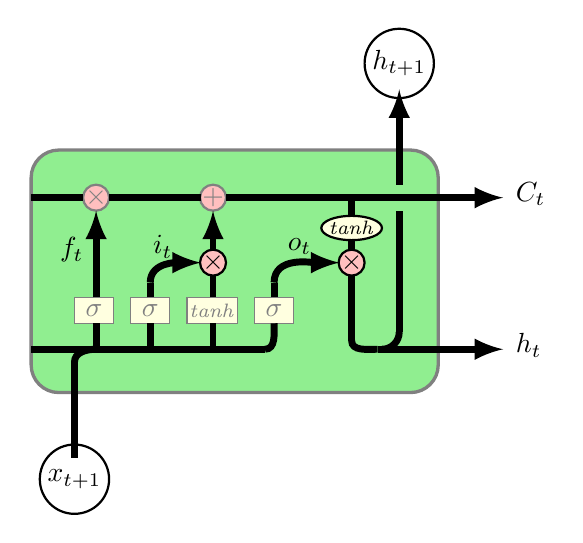
\begin{tikzpicture}[scale=1.1]

  % The grid
  % \draw[step=0.5, gray!40, very thin] (0,0) grid (8,4);

  % LSTM frame
  \def \yONE {0.5}
  \def \yTWO {3.3}
  \draw[rounded corners=10pt, very thick, gray,fill=LightGreen]  (1.5, 0.5) rectangle (6.2, 3.3);

  \def \sigmoidWidth  {0.45}
  \def \sigmoidInDist {0.2}
  \def \sigmoidHeight  {0.3}
  \def \yB  {1.3}
  \def \yD  {2.75}
  \def \shift {0.3}
  % First Sigmoid
  \draw[gray,fill=LightYellow] (2, \yB) rectangle (2+ \sigmoidWidth, \yB + \sigmoidHeight) node[pos=0.5] {$\sigma$};

  \def \r {.15cm}
  % The Upper times operator % first time from left
  \draw[thick, gray,fill=pink] (2.25, \yD) circle (\r) node {$\times$};

  % Second Sigmoid
  \def \xS {2.45 +\sigmoidInDist}
  \draw[gray,fill=LightYellow]  (\xS, \yB) rectangle (\xS +\sigmoidWidth, \yB + \sigmoidHeight) node[pos=0.5] {$\sigma$};

  % Square tanh
  \def \xSS {\xS +\sigmoidWidth + \sigmoidInDist}
  \draw[gray,fill=LightYellow]  (\xSS, \yB) 
  rectangle 
  (\xSS +\sigmoidWidth +0.13, \yB +\sigmoidHeight)
  node[pos=0.5] {\scriptsize \textit{tanh}};

  % Third Sigoid
  \def \xSSS {\xSS +\sigmoidWidth +0.13 +\sigmoidInDist}
  \draw[gray,fill=LightYellow]  (\xSSS, \yB) rectangle (\xSSS +\sigmoidWidth, \yB +\sigmoidHeight)
  node[pos=0.5] { $\sigma$};

  % Second times operator and add operator
  \def \xTimesB {3.6}
  \def \yC      {2}

  \draw[thick,fill=pink] (\xTimesB, \yC) circle (\r) node {$\times$};
  %%%%% first line sectond operator +
  \draw[thick, gray,fill=pink] (\xTimesB, \yD) circle (\r) node {$+$};

  % Third times operator and its tanh
  \draw[thick,fill=pink] (\xTimesB +1.3 +\shift, \yC) circle (\r) node {$\times$};
  \draw[thick,fill=LightYellow] (\xTimesB +1.3 +\shift, \yC +.4)  
  ellipse (.35cm and .14cm) 
  node {\scriptsize \textit{tanh}};


  % LINES %%% Upper line from c_{t -1} till C_t
  %\draw[arrows=-latex, line width=2.5pt]  (0.85, \yD) -- (1.5, \yD) node[left, xshift=-.6cm, yshift=0.2cm] {$C_{t-1}$};
  \draw[line width=2.5pt]  (1.5, \yD) -- (2.1, \yD);
  \draw[line width=2.5pt]  (2.4, \yD) -- (3.46, \yD);
  \draw[line width=2.5pt]  (3.75, \yD) -- (6.25 +0.2, \yD);

  \draw[arrows=-latex, line width=2.5pt]  (6.25, \yD) -- (6.75 +0.2, \yD)
  node[right, xshift=0.0cm, yshift=0.05cm] {$C_t$};

  %%%%first line from left from sigmoid ft till times input from C_{t-1}
  \draw[arrows=-latex, line width=2.5pt]  (2.25, \yB +\sigmoidHeight) -- (2.25, 2.6)
  node[left, yshift=-0.5cm] {$f_t$};

  % Level B LINES
  \def \levelB {1}
  %\draw[arrows=-latex, line width=2.5pt] (0.85, \levelB) -- (1.5, \levelB) node[left, xshift=-.6cm, yshift=0.2cm] {$h_{t-1}$};

  \draw[line width=2.5pt] (1.5, \levelB) 
  --
  (4.2, \levelB);

  \def \xOfThirdSigmoid {\xSSS + \sigmoidWidth/2}
  %second line last angle connected to sigmoid 
  \draw[line width=2.5pt] (4.2, \levelB) to[out=0,in=270] (\xOfThirdSigmoid, \yB);

  % Third Sigmoid up line
  % END (\xTimesB +1.3 - 0.19 , \yC)
  \draw[line width=2.5pt] (\xOfThirdSigmoid, \yB + \sigmoidHeight) 
  --
  (\xOfThirdSigmoid, \yB + \sigmoidHeight + 0.17) ;

  \draw[arrows=-latex, line width=2.5pt] (\xOfThirdSigmoid, \yB + \sigmoidHeight+0.17) 
  to[out=90, in=180] 
  (\xTimesB +1.3 -0.14 +\shift , \yC) 
  node [left, yshift=0.2cm, xshift=-0.2cm] {$o_t$};

  % tanh line
  \draw [line width=2.5pt] (\xTimesB, \levelB)
  --
  (\xTimesB, \yB);

  \draw [line width=2.5pt] (\xTimesB, \yB + \sigmoidHeight)
  --
  (\xTimesB, \yB + \sigmoidHeight +0.24);

  \draw [arrows=-latex, line width=2.5pt] (\xTimesB, 2.15)
  --
  (\xTimesB, 2.6);

  \draw[line width=2.5pt] (2.25, \levelB)
  --
  (2.25, \yB);
  
  \draw[line width=2.5pt] (\xS +\sigmoidWidth/2, \levelB)
  --
  (\xS +\sigmoidWidth/2, \yB);

  \draw[line width=2.5pt] (\xS +\sigmoidWidth/2, \yB +\sigmoidHeight)
  -- 
  (\xS +\sigmoidWidth/2, \yB +\sigmoidHeight + 0.17);

  \draw[arrows=-latex, line width=2.5pt] (\xS +\sigmoidWidth/2, \yB + \sigmoidHeight+0.17) 
  to[out=90, in=180] 
  (\xTimesB-0.14, \yC)
  node [left, yshift=0.2cm, xshift=-0.2cm] {$i_t$};

  \def \bigR {0.25cm}
  \def \bigRTWO {0.4cm}
  \def \C    {1}
  \def \xBigCicleONE {2}
  \def \xBigCicleTWO {5.5 + 0.25}
  \draw[thick] (\xBigCicleONE, \yONE - \C) circle (\bigRTWO) node {$x_{t+1}$};
  \draw[thick] (\xBigCicleTWO, \yTWO + \C) circle (\bigRTWO) node {$h_{t+1}$};

  % LINE Circle ONE
  \draw[line width=2.5pt] (\xBigCicleONE, \yONE -\C +0.25) 
  --
  (\xBigCicleONE, \yONE -\C +0.25 + 1.1);

  \draw[line width=2.5pt] (\xBigCicleONE, \yONE -\C +0.25 + 1.1)
  to[out=90, in=180]
  (2.25, 1);

  % LINE third \times
  \draw[line width=2.5pt] (\xTimesB +1.3 +\shift, 1.1)
  --
  (\xTimesB +1.3 +\shift, \yC - 0.15);

  \draw[line width=2.5pt] (5.5, 1) 
  --
  (6.25 +0.2, 1);
  
  \draw[arrows=-latex, line width=2.5pt] (6.25, 1) 
  --
  (6.75 +0.2, 1)
  node[right, xshift=0.0cm, yshift=0.05cm,] {$h_t$};

%%% second line last angle connect the input with h_t output
  \draw[line width=2.5pt] (\xTimesB +1.3 +\shift, 1.1)
  to[out=270, in=180]
  (5.5, 1);


  \draw[line width=2.5pt] (\xTimesB +1.3 +\shift, 2.14)
  --
  (\xTimesB +1.3 +\shift, 2.26);


  \draw[line width=2.5pt] (\xTimesB +1.3 +\shift, \yD)
  --
  (\xTimesB +1.3 +\shift, 2.54);


  \draw[line width=2.5pt] (\xBigCicleTWO, \levelB +0.2)
  --
  (\xBigCicleTWO, 2.6);

%%%%% first horizontal line from the right angle connected to output ht
  \draw[line width=2.5pt] (\xBigCicleTWO - 0.2, \levelB)
  to[out=0, in=270]
  (\xBigCicleTWO, \levelB +0.2);


  \draw[arrows=-latex, line width=2.5pt]
  (\xBigCicleTWO, \yD +0.15)
  --
  (\xBigCicleTWO, 4);

\end{tikzpicture}


	\endminipage\hfill
	\minipage{0.33\textwidth}%
	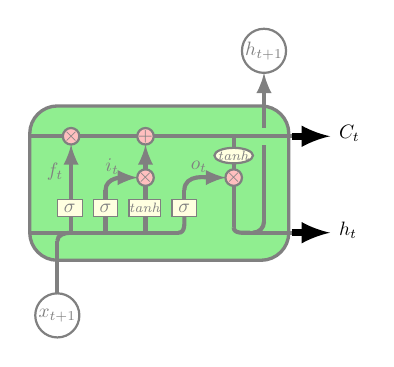
\begin{tikzpicture}[scale=.7, transform shape]

  % The grid
  % \draw[step=0.5, gray!40, very thin] (0,0) grid (8,4);

  % LSTM frame
  \def \yONE {0.5}
  \def \yTWO {3.3}
  \draw[rounded corners=10pt, very thick, gray,fill=LightGreen]  (1.5, 0.5) rectangle (6.2, 3.3);

  \def \sigmoidWidth  {0.45}
  \def \sigmoidInDist {0.2}
  \def \sigmoidHeight  {0.3}
  \def \yB  {1.3}
  \def \yD  {2.75}
  \def \shift {0.3}
  % First Sigmoid
  \draw[gray,fill=LightYellow] (2, \yB) rectangle (2+ \sigmoidWidth, \yB + \sigmoidHeight) node[pos=0.5] {$\sigma$};

  \def \r {.15cm}
  % The Upper times operator % first time from left
  \draw[thick, gray,fill=pink] (2.25, \yD) circle (\r) node {$\times$};

  % Second Sigmoid
  \def \xS {2.45 +\sigmoidInDist}
  \draw[gray,fill=LightYellow]  (\xS, \yB) rectangle (\xS +\sigmoidWidth, \yB + \sigmoidHeight) node[pos=0.5] {$\sigma$};

  % Square tanh
  \def \xSS {\xS +\sigmoidWidth + \sigmoidInDist}
  \draw[gray,fill=LightYellow]  (\xSS, \yB) 
  rectangle 
  (\xSS +\sigmoidWidth +0.13, \yB +\sigmoidHeight)
  node[pos=0.5] {\scriptsize \textit{tanh}};

  % Third Sigoid
  \def \xSSS {\xSS +\sigmoidWidth +0.13 +\sigmoidInDist}
  \draw[gray,fill=LightYellow]  (\xSSS, \yB) rectangle (\xSSS +\sigmoidWidth, \yB +\sigmoidHeight)
  node[pos=0.5] { $\sigma$};

  % Second times operator and add operator
  \def \xTimesB {3.6}
  \def \yC      {2}

  \draw[thick,gray,fill=pink] (\xTimesB, \yC) circle (\r) node {$\times$};
  %%%%% first line sectond operator +
  \draw[thick, gray,fill=pink] (\xTimesB, \yD) circle (\r) node {$+$};

  % Third times operator and its tanh
  \draw[thick,gray,fill=pink] (\xTimesB +1.3 +\shift, \yC) circle (\r) node {$\times$};
  \draw[thick,gray,fill=LightYellow] (\xTimesB +1.3 +\shift, \yC +.4)  
  ellipse (.35cm and .14cm) 
  node {\scriptsize \textit{tanh}};


  % LINES %%% Upper line from c_{t -1} till C_t
  %\draw[arrows=-latex, line width=2.5pt]  (0.85, \yD) -- (1.5, \yD) node[left, xshift=-.6cm, yshift=0.2cm] {$C_{t-1}$};
  \draw[line width=1.5pt,gray]  (1.5, \yD) -- (2.1, \yD);
  \draw[line width=1.5pt,gray]  (2.4, \yD) -- (3.46, \yD);
  \draw[line width=1.5pt,gray]  (3.75, \yD) -- (6.25 +0.2, \yD);

  \draw[arrows=-latex, line width=2.5pt]  (6.25, \yD) -- (6.75 +0.2, \yD)
  node[right, xshift=0.0cm, yshift=0.05cm] {$C_t$};

  %%%%first line from left from sigmoid ft till times input from C_{t-1}
  \draw[arrows=-latex, line width=1.5pt,gray]  (2.25, \yB +\sigmoidHeight) -- (2.25, 2.6)
  node[left, yshift=-0.5cm] {$f_t$};

  % Level B LINES
  \def \levelB {1}
  %\draw[arrows=-latex, line width=1.5pt,gray] (0.85, \levelB) -- (1.5, \levelB) node[left, xshift=-.6cm, yshift=0.2cm] {$h_{t-1}$};

  \draw[line width=1.5pt,gray] (1.5, \levelB) 
  --
  (4.2, \levelB);

  \def \xOfThirdSigmoid {\xSSS + \sigmoidWidth/2}
  %second line last angle connected to sigmoid 
  \draw[line width=1.5pt,gray] (4.2, \levelB) to[out=0,in=270] (\xOfThirdSigmoid, \yB);

  % Third Sigmoid up line
  % END (\xTimesB +1.3 - 0.19 , \yC)
  \draw[line width=1.5pt,gray] (\xOfThirdSigmoid, \yB + \sigmoidHeight) 
  --
  (\xOfThirdSigmoid, \yB + \sigmoidHeight + 0.17) ;

  \draw[arrows=-latex, line width=1.5pt,gray] (\xOfThirdSigmoid, \yB + \sigmoidHeight+0.17) 
  to[out=90, in=180] 
  (\xTimesB +1.3 -0.14 +\shift , \yC) 
  node [left, yshift=0.2cm, xshift=-0.2cm] {$o_t$};

  % tanh line
  \draw [line width=1.5pt,gray] (\xTimesB, \levelB)
  --
  (\xTimesB, \yB);

  \draw [line width=1.5pt,gray] (\xTimesB, \yB + \sigmoidHeight)
  --
  (\xTimesB, \yB + \sigmoidHeight +0.24);

  \draw [arrows=-latex, line width=1.5pt,gray] (\xTimesB, 2.15)
  --
  (\xTimesB, 2.6);

  \draw[line width=1.5pt,gray] (2.25, \levelB)
  --
  (2.25, \yB);
  
  \draw[line width=1.5pt,gray] (\xS +\sigmoidWidth/2, \levelB)
  --
  (\xS +\sigmoidWidth/2, \yB);

  \draw[line width=1.5pt,gray] (\xS +\sigmoidWidth/2, \yB +\sigmoidHeight)
  -- 
  (\xS +\sigmoidWidth/2, \yB +\sigmoidHeight + 0.17);

  \draw[arrows=-latex, line width=1.5pt,gray] (\xS +\sigmoidWidth/2, \yB + \sigmoidHeight+0.17) 
  to[out=90, in=180] 
  (\xTimesB-0.14, \yC)
  node [left, yshift=0.2cm, xshift=-0.2cm] {$i_t$};

  \def \bigR {0.25cm}
  \def \bigRTWO {0.4cm}
  \def \C    {1}
  \def \xBigCicleONE {2}
  \def \xBigCicleTWO {5.5 + 0.25}
  \draw[thick,gray] (\xBigCicleONE, \yONE - \C) circle (\bigRTWO) node {$x_{t+1}$};
  \draw[thick,gray] (\xBigCicleTWO, \yTWO + \C) circle (\bigRTWO) node {$h_{t+1}$};

  % LINE Circle ONE
  \draw[line width=1.5pt,gray] (\xBigCicleONE, \yONE -\C +0.4) 
  --
  (\xBigCicleONE, \yONE -\C +0.25 + 1.1);

  \draw[line width=1.5pt,gray] (\xBigCicleONE, \yONE -\C +0.25 + 1.1)
  to[out=90, in=180]
  (2.25, 1);

  % LINE third \times
  \draw[line width=1.5pt,gray] (\xTimesB +1.3 +\shift, 1.1)
  --
  (\xTimesB +1.3 +\shift, \yC - 0.15);

  \draw[line width=1.5pt,gray] (5.5, 1) 
  --
  (6.25 +0.2, 1);
  
  \draw[arrows=-latex,line width=2.5pt] (6.25, 1) 
  --
  (6.75 +0.2, 1)
  node[right, xshift=0.0cm, yshift=0.05cm,] {$h_t$};

%%% second line last angle connect the input with h_t output
  \draw[line width=1.5pt,gray] (\xTimesB +1.3 +\shift, 1.1)
  to[out=270, in=180]
  (5.5, 1);


  \draw[line width=1.5pt,gray] (\xTimesB +1.3 +\shift, 2.14)
  --
  (\xTimesB +1.3 +\shift, 2.26);


  \draw[line width=1.5pt,gray] (\xTimesB +1.3 +\shift, \yD)
  --
  (\xTimesB +1.3 +\shift, 2.54);


  \draw[line width=1.5pt,gray] (\xBigCicleTWO, \levelB +0.2)
  --
  (\xBigCicleTWO, 2.6);

%%%%% first horizontal line from the right angle connected to output ht
  \draw[line width=1.5pt,gray] (\xBigCicleTWO - 0.2, \levelB)
  to[out=0, in=270]
  (\xBigCicleTWO, \levelB +0.2);


  \draw[arrows=-latex, line width=1.5pt,gray]
  (\xBigCicleTWO, \yD +0.15)
  --
  (\xBigCicleTWO, 4-.1);

\end{tikzpicture}

	\endminipage
	\caption{Unfold LSTM adapted from~\cite{colah}}
	~\label{Fig:LSTM_Cell_Chaining}
\end{figure}%
\end{frame}

%%%%%%%%%%%%%%%%%%%%%%%%%%%%%%%%%%%%%%%%%%%%%%%%%%

\begin{frame}[fragile]{LSTM Architectures}
\begin{block}{Bi-LSTM Motivation}
		\begin{itemize}
	\item[--] \textit{\textbf{Harry}} is the king, and he will travel next week.
	\item[--] The new book which makes the big sale is named \textit{\textbf{Harry}} Potter.
\end{itemize}
\end{block}

\begin{itemize}
	\item Bi-LSTM models always outperform LSTM models.
	\item It means that models can't learn the pattern from one direction, it
	should be two directions together.
\end{itemize}
\end{frame}
%%%%%%%%%%%%%%%%%%%%%%%%%%%%%%%%%%%%%%%%%%%%%%%%%%

\begin{frame}[fragile]{LSTM Architectures}
\begin{center}
\begin{figure}[!t]
\centering
\begin{tikzpicture}[scale=.6, transform shape]
	\node[rectangle] (Y0) at (0, 0) {$\dots$};
	\node[rectangle, draw, right=2em of Y0, minimum height=1cm, minimum width=1cm] (RNN) {LSTM$_\rightarrow$};
	\node[rectangle, right=of RNN, draw, minimum height=1cm, minimum width=1cm] (RNN2) {LSTM$_\rightarrow$};
	\node[rectangle, right=of RNN2, draw, minimum height=1cm, minimum width=1cm] (RNN3) {LSTM$_\rightarrow$};
			
	\node[rectangle, right= of RNN3, draw, minimum height=1cm, minimum width=1cm] (RNN4) {LSTM$_\rightarrow$};
	\node[rectangle, right=2em of RNN4] (RNN5) {$\dots$};
			
			
	\node[rectangle, above=of RNN4, draw, minimum height=1cm, minimum width=1cm] (R25) {LSTM$_\leftarrow$};
	\node[rectangle, left=of R25, minimum height=1cm, minimum width=1cm, draw] (R24) {LSTM$_\leftarrow$};
	\node[rectangle, left=of R24, draw, minimum height=1cm, minimum width=1cm] (R23) {LSTM$_\leftarrow$};
	\node[rectangle, left=of R23, draw, minimum height=1cm, minimum width=1cm] (R22) {LSTM$_\leftarrow$};
	\node[rectangle, left=2em of R22] (R21) {$\dots$};
	\node[right=2em of R25] (Y20) {$\dots$};
			
	\node[below=of RNN] (X1) {$\vec{x}_2$};
	\node[below=of RNN2] (X2) {$\vec{x}_3$};
	\node[below=of RNN3] (X3) {$\vec{x}_4$};
	\node[below=of RNN4] (X4) {$\vec{x}_5$};
	\node[above=of R25] (Y5) {$\vec{h}_5$};
	\node[above=of R24] (Y4) {$\vec{h}_4$};
	\node[above=of R23] (Y3) {$\vec{h}_3$};
	\node[above=of R22] (Y2) {$\vec{h}_2$};
			
	\draw[-stealth, thick] (X1) -- (RNN);
	\draw[-stealth, thick] (X2) -- (RNN2);
	\draw[-stealth, thick] (X3) -- (RNN3);
	\draw[-stealth, thick] (X4) -- (RNN4);
	\draw[-stealth, thick, densely dotted] (Y0) -- (RNN);
	\draw[-stealth, thick] (RNN) -- node[above, pos=0.35] {$\vec{h}_2^\rightarrow$} (RNN2);
	\draw[-stealth, thick] (RNN2) -- node[above, pos=0.35] {$\vec{h}_3^\rightarrow$} (RNN3);
	\draw[-stealth, thick] (RNN3) -- node[above, pos=0.35] {$\vec{h}_4^\rightarrow$} (RNN4);
	\draw[-stealth, densely dotted, thick] (RNN4) -- (RNN5);
	\node[below=4em of Y0] (d) {\dots};
	\node[below=4em of RNN5] (d) {\dots};
			
	\path[-stealth, ultra thick, white] (X1) edge[bend left=45] (R22);
	\path[-stealth, thick] (X1) edge[bend left=45] (R22);
	\path[-stealth, ultra thick, white] (X2) edge[bend left=45] (R23);
	\path[-stealth, thick] (X2) edge[bend left=45] (R23);
	\path[-stealth, ultra thick, white] (X3) edge[bend left=45] (R24);
	\path[-stealth, thick] (X3) edge[bend left=45] (R24);
	\path[-stealth, ultra thick, white] (X4) edge[bend left=45] (R25);
	\path[-stealth, thick] (X4) edge[bend left=45] (R25);
	\draw[-stealth, densely dotted, thick] (Y20) -- (R25);
			
	\draw[-stealth, thick] (R22) -- (Y2);
	\draw[-stealth, thick] (R23) -- (Y3);
	\draw[-stealth, thick] (R24) -- (Y4);
	\draw[-stealth, thick] (R25) -- (Y5);
		
	\draw[stealth-, densely dotted, thick] (R21) -- (R22);
	\draw[stealth-, thick] (R22) -- node[above, pos=0.65] {$\vec{h}_3^\leftarrow$} (R23);
	\draw[stealth-, thick] (R23) -- node[above, pos=0.65] {$\vec{h}_4^\leftarrow$} (R24);
	\draw[stealth-, thick] (R24) -- node[above, pos=0.65] {$\vec{h}_5^\leftarrow$} (R25);
	\draw[-stealth, densely dotted, thick] (Y20) -- (R25);	
			
	\path[-stealth, ultra thick, white] (RNN) edge[bend right=45] (Y2);
	\path[-stealth, thick] (RNN) edge[bend right=45] (Y2);
	\path[-stealth, ultra thick, white] (RNN2) edge[bend right=45] (Y3);
	\path[-stealth, thick] (RNN2) edge[bend right=45] (Y3);
	\path[-stealth, ultra thick, white] (RNN3) edge[bend right=45] (Y4);
	\path[-stealth, thick] (RNN3) edge[bend right=45] (Y4);
	\path[-stealth, ultra thick, white] (RNN4) edge[bend right=45] (Y5);
	\path[-stealth, thick] (RNN4) edge[bend right=45] (Y5);
			
\end{tikzpicture}

\caption{bidirectional long short-term memory~\cite{Gitrepo_NN_Tikz}}~\label{Fig:BI-LSTM}
\end{figure}
\end{center}
\end{frame}
%%%%%%%%%%%%%%%%%%%%%%%%%%%%%%%%%%%%%%%%%%%%%%%%%%
%%%%%%%%%%%%%%%%%%%%%%%%%%%%%%%%%%%%%%%%%%%%%%%%%%
%%%%%%%%%%%%%%%%%%%%%%%%%%%%%%%%%%%%%%%%%%%%%%%%%%

\section{Experiments and Results}

%%%%%%%%%%%%%%%%%%%%%%%%%%%%%%%%%%%%%%%%%%%%%%%%%%
\begin{frame}[fragile]{Experiments Parameters}
\begin{itemize}
	\item \textbf{Dataset Configurations}:
	\begin{itemize}
		\item [-] Encoding technique: BinE, OneE, TwoE.
		\item [-] Diacritics: 0D, 1D.
		\item [-] Trimming: 0T, 1T.
	\end{itemize}
\item \textbf{Network Configurations}:
\begin{itemize}
\item [-] Loss functions: \textit{Weighted} or \textit{Non-Weighted } \textbf{(1, 0)} respectively.
\item [-] The number of layers: nL.
\item [-] The number of cell units: nU.
\item [-] Cell type: LSTM, Bi-LSTM.
\end{itemize}
\end{itemize}
\end{frame}

%%%%%%%%%%%%%%%%%%%%%%%%%%%%%%%%%%%%%%%%%%%%%%%%%%
\begin{frame}[fragile]{Overall Accuracy!}
\Wider{
\begin{figure}[!t]
	\begin{tikzpicture}[scale=.95, transform shape]
  %% Uses pointModelsFiguresStyle macro defined in pgfplot_configurations.tex

  %% two grid to help during positioing.
  % \draw[step=0.2, green!40, thin] (0,0) grid (8,6);
  % \draw[step=1, red!40, very thin] (0,-1) grid (8,7);

  %% Variables
  \def \maxHeight{5.7}
  \def \yONE{-0.8}
  \def \yTWO{-0.3}

  %% two colored areas to distinguish the diacritic models.
  \fill[gray!30, opacity=0.2, rounded corners=2pt] (0,-0.5) rectangle (2.1,\maxHeight);
  \fill[gray!30, opacity=0.2, rounded corners=2pt] (4.2,-0.5) rectangle (6.32,\maxHeight);

  %% The Full/Elimenated Seperator
  \draw[dashed, thick] (4.2, 0 - 0.9) -- (4.2, \maxHeight +0.5);

  %% Group Labels Full/Elimenated
  \node [align=center, text width=3cm, inner sep=0.25cm] at (2.1, \yONE) {\scriptsize no trimming(0T)};
  \node [align=center, text width=4cm, inner sep=0.25cm] at (6.32,\yONE) {\scriptsize trimming(1T)};

  \node [align=center, text width=3cm, inner sep=0.25cm] at (1, \yTWO) {\scriptsize diacritic(1D)};
  \node [align=center, text width=3cm, inner sep=0.25cm] at (3, \yTWO) {\scriptsize no diacritic(0D)};
  \node [align=center, text width=3cm, inner sep=0.25cm] at (5+0.2, \yTWO) {\scriptsize diacritic(1D)};
  \node [align=center, text width=3cm, inner sep=0.25cm] at (7+0.2, \yTWO) {\scriptsize no diacritic(0D)};

  % Points annotaions
  \def \layerHeight{5.7}
  \def \unitHeight{\layerHeight - 0.3}
  \def \weightedHeihgt{\layerHeight - 0.6}

  \def \step{0.2}
  \def \move{0.1}
  %%%%%% 

  \node  at (3.5*   \step -0.15-\move, \layerHeight) {\scriptsize 7L};
  \node  at (3.5*   \step -0.15-\move, \unitHeight) {\scriptsize 82U};
  \node  at (3.5*   \step -0.1 -\move, \weightedHeihgt) {\scriptsize 0};

  \node  at (5.2*   \step, \layerHeight) {\scriptsize 7L};
  \node  at (5.2*   \step, \unitHeight) {\scriptsize 50U};
  \node  at (5.2*   \step, \weightedHeihgt) {\scriptsize 1};

  \node  at (7*     \step +0.15+\move, \layerHeight) {\scriptsize 7L};
  \node  at (7*   \step   +0.15+\move, \unitHeight) {\scriptsize 50U};
  \node  at (7*   \step   +0.1 +\move, \weightedHeihgt) {\scriptsize 1};

  %%%%%%

  \node  at (14*    \step -0.15-\move, \layerHeight) {\scriptsize 7L};
  \node  at (14*   \step -0.15 -\move, \unitHeight) {\scriptsize 82U};
  \node  at (14*   \step -0.1  -\move, \weightedHeihgt) {\scriptsize 0};

  \node  at (16*    \step, \layerHeight) {\scriptsize 7L};
  \node  at (16*    \step, \unitHeight) {\scriptsize 82U};
  \node  at (16*    \step, \weightedHeihgt) {\scriptsize 0};

  \node  at (17.6*  \step +0.15+\move, \layerHeight) {\scriptsize 7L};
  \node  at (17.6*  \step +0.15+\move, \unitHeight) {\scriptsize 50U};
  \node  at (17.6*  \step +0.1 +\move, \weightedHeihgt) {\scriptsize 0};

  %%%%%%

  \node  at (24.5*  \step -0.15-\move, \layerHeight) {\scriptsize 7L};
  \node  at (24.5*  \step -0.15-\move, \unitHeight) {\scriptsize 82U};
  \node  at (24.5*  \step -0.1 -\move,  \weightedHeihgt) {\scriptsize 1};

  \node  at (26.1*  \step, \layerHeight) {\scriptsize 7L};
  \node  at (26.1*  \step, \unitHeight) {\scriptsize 82U};
  \node  at (26.1*  \step, \weightedHeihgt) {\scriptsize 0};

  \node  at (28*    \step +0.15+\move, \layerHeight) {\scriptsize 7L};
  \node  at (28*    \step +0.15+\move, \unitHeight) {\scriptsize 82U};
  \node  at (28*    \step +0.1 +\move,  \weightedHeihgt) {\scriptsize 1};

  %%%%%%

  \node  at (35*    \step -0.15-\move, \layerHeight) {\scriptsize 4L};
  \node  at (35*    \step -0.15-\move, \unitHeight) {\scriptsize 82U};
  \node  at (35*    \step -0.1 -\move,  \weightedHeihgt) {\scriptsize 0};

  \node  at (37*    \step, \layerHeight) {\scriptsize 7L};
  \node  at (37*    \step, \unitHeight) {\scriptsize 82U};
  \node  at (37*    \step, \weightedHeihgt) {\scriptsize 0};

  \node  at (38.7*  \step +0.15+\move, \layerHeight) {\scriptsize 4L};
  \node  at (38.7*  \step +0.15+\move, \unitHeight) {\scriptsize 50U};
  \node  at (38.7*  \step +0.1 +\move,  \weightedHeihgt) {\scriptsize 1};

  \begin{axis}[
    major x tick style = transparent,
    ybar=2*\pgflinewidth,
    x=10pt,
    ymajorgrids = true,
    % every axis y label/.style= {at={( 0, 1.09)}, anchor=north},
    ylabel = {Accuracy},
    ylabel style = {font=\footnotesize},
    xtickmin={1},
    xtickmax={21},
    axis x line = bottom,
    axis y line = left,
    enlarge y limits={upper, value=0.1},
    xticklabels = {,,},
    bar shift=0pt,
    % scaled y ticks = false,
    enlarge x limits=0.1,
    ymin=0.76,
    ymax=0.98,
    legend style={at={(0.5, -0.4)}, anchor=north, legend columns=3},
    % legend style={at={(0.9, 0.26)}, anchor=north, legend columns=1},
    every axis legend/.append style={nodes={right}},
    nodes near coords={\vspace*{0.1\baselineskip}
      \foreach \X in \pgfplotspointmeta%
      {\centerline{\X}\newline}%
      \vspace*{-0.7\baselineskip}
    },
    nodes near coords style={font=\scriptsize,anchor=-90, text width=1cm},
    ]


    % Binary
    \addplot[pointBiLSTM=blue] coordinates {

    % BLSTM
    (1, 0.9025442765600247) % Exp_7_T1_D1_binary_BLSTM_6_82_0
    (7, 0.8766640656404435) % Exp_7_T1_D0_binary_BLSTM_6_82_0
    (13, 0.8988593838876747) % Exp_8_T0_D1_binary_BLSTM_6_82_1
    (19, 0.9638475586025206) % Exp_3_T0_D0_binary_BLSTM_3_82_0
    };

    % Binary
    \addplot[pointLSTM=blue] coordinates {
    % LSTM
    (1, 0.7977761225792721) % Exp_11_T1_D1_binary_LSTM_3_82_0
    (7, 0.7883237568276937) % Exp_13_T1_D0_binary_LSTM_6_50_0
    (13, 0.827841810615813) % Exp_15_T0_D1_binary_LSTM_6_82_0
    (19, 0.816387749603329) % Exp_12_T0_D0_binary_LSTM_3_82_1
    };

    % OneHot
    \addplot[pointBiLSTM=red] coordinates {
    (2, 0.9346846846846846) % Exp_6_T1_D1_onehot_BLSTM_6_50_1
    (8, 0.9310432479723819) % Exp_7_T1_D0_onehot_BLSTM_6_82_0
    (14, 0.9472562344699578) % Exp_7_T0_D1_onehot_BLSTM_6_82_0
    (20, 0.9280962787773555) % Exp_7_T0_D0_onehot_BLSTM_6_82_0
    };

    % OneHot
    \addplot[pointLSTM=red] coordinates {
    (2, 0.8965678276701898) % Exp_11_T1_D1_onehot_LSTM_3_82_0
    (8, 0.8869854106074577) % Exp_9_T1_D0_onehot_LSTM_3_50_0
    (14, 0.9094811843247613) % Exp_12_T0_D1_onehot_LSTM_3_82_1
    (20, 0.9219171930664911) % Exp_15_T0_D0_onehot_LSTM_6_82_0
    };

    % TwoHot
    \addplot[pointBiLSTM=brown] coordinates {
    (3, 0.9458158946347922) % Exp_6_T1_D1_twohot_BLSTM_6_50_1
    (9, 0.9411340474332599) % Exp_5_T1_D0_twohot_BLSTM_6_50_0
    (15, 0.954692692273149) % Exp_8_T0_D1_twohot_BLSTM_6_82_1
    (21, 0.9628835733317367) % Exp_2_T0_D0_twohot_BLSTM_3_50_1
    };

    % TwoHowt
    \addplot[pointLSTM=brown] coordinates {
    (3, 0.9170331749071906) % Exp_12_T1_D1_twohot_LSTM_3_82_1
    (9, 0.8972239956491926) % Exp_9_T1_D0_twohot_LSTM_3_50_0
    (15, 0.94120887345448) % Exp_11_T0_D1_twohot_LSTM_3_82_0
    (21, 0.9284854653773613) % Exp_12_T0_D0_twohot_LSTM_3_82_1
    };




    %%%%%%%%%%%%%%%%%%%%%
    %% The rest models
    %%%%%%%%%%%%%%%%%%%%%
    % Binary
    \addplot[pointRug=blue, mark size=0.7pt]
    coordinates {
      % 1, 7, 13, 19

%
(1, 0.861495353621338) % Exp_2_T1_D1_binary_BLSTM_3_50_1
(1, 0.866862925918044) % Exp_4_T1_D1_binary_BLSTM_3_82_1
(1, 0.867725993710246) % Exp_1_T1_D1_binary_BLSTM_3_50_0
(1, 0.8706225910950319) % Exp_5_T1_D1_binary_BLSTM_6_50_0
(1, 0.8794601688302476) % Exp_6_T1_D1_binary_BLSTM_6_50_1
(1, 0.8869558534912864) % Exp_3_T1_D1_binary_BLSTM_3_82_0
(1, 0.8948003121231469) % Exp_8_T1_D1_binary_BLSTM_6_82_1
(1, 0.9025442765600247) % Exp_7_T1_D1_binary_BLSTM_6_82_0

(1, 0.23921165259747937) % Exp_10_T1_D1_binary_LSTM_3_50_1
(1, 0.23921165259747937) % Exp_12_T1_D1_binary_LSTM_3_82_1
(1, 0.23921165259747937) % Exp_13_T1_D1_binary_LSTM_6_50_0
(1, 0.23921165259747937) % Exp_15_T1_D1_binary_LSTM_6_82_0
(1, 0.5386134165661725) % Exp_16_T1_D1_binary_LSTM_6_82_1
(1, 0.6374642358894328) % Exp_9_T1_D1_binary_LSTM_3_50_0
(1, 0.6666016410110899) % Exp_14_T1_D1_binary_LSTM_6_50_1
(1, 0.7977761225792721) % Exp_11_T1_D1_binary_LSTM_3_82_0

%
(7, 0.7722328627840438) % Exp_2_T1_D0_binary_BLSTM_3_50_1
(7, 0.7918174079591402) % Exp_6_T1_D0_binary_BLSTM_6_50_1
(7, 0.7977524768863351) % Exp_1_T1_D0_binary_BLSTM_3_50_0
(7, 0.8173251992149632) % Exp_5_T1_D0_binary_BLSTM_6_50_0
(7, 0.8267420964271357) % Exp_4_T1_D0_binary_BLSTM_3_82_1
(7, 0.8307795984961339) % Exp_8_T1_D0_binary_BLSTM_6_82_1
(7, 0.8564115296398761) % Exp_3_T1_D0_binary_BLSTM_3_82_0
(7, 0.8766640656404435) % Exp_7_T1_D0_binary_BLSTM_6_82_0


(7, 0.23921165259747937) % Exp_10_T1_D0_binary_LSTM_3_50_1
(7, 0.23921165259747937) % Exp_12_T1_D0_binary_LSTM_3_82_1
(7, 0.23921165259747937) % Exp_15_T1_D0_binary_LSTM_6_82_0
(7, 0.5082878153744296) % Exp_14_T1_D0_binary_LSTM_6_50_1
(7, 0.7268331323449435) % Exp_11_T1_D0_binary_LSTM_3_82_0
(7, 0.7272055520087017) % Exp_9_T1_D0_binary_LSTM_3_50_0
(7, 0.7346362110141638) % Exp_16_T1_D0_binary_LSTM_6_82_1
(7, 0.7883237568276937) % Exp_13_T1_D0_binary_LSTM_6_50_0

%
(13, 0.8288896206927522) % Exp_1_T0_D1_binary_BLSTM_3_50_0
(13, 0.8555698589947012) % Exp_4_T0_D1_binary_BLSTM_3_82_1
(13, 0.8634134658563603) % Exp_2_T0_D1_binary_BLSTM_3_50_1
(13, 0.8649043499086908) % Exp_3_T0_D1_binary_BLSTM_3_82_0
(13, 0.8741370535580637) % Exp_6_T0_D1_binary_BLSTM_6_50_1
(13, 0.8841181929766787) % Exp_7_T0_D1_binary_BLSTM_6_82_0
(13, 0.8986558093584409) % Exp_5_T0_D1_binary_BLSTM_6_50_0
(13, 0.8988593838876747) % Exp_8_T0_D1_binary_BLSTM_6_82_1

(13, 0.6457563691883963) % Exp_10_T0_D1_binary_LSTM_3_50_1
(13, 0.740628087297548) % Exp_13_T0_D1_binary_LSTM_6_50_0
(13, 0.7581235218393557) % Exp_16_T0_D1_binary_LSTM_6_82_1
(13, 0.7709068047780139) % Exp_11_T0_D1_binary_LSTM_3_82_0
(13, 0.7879471903721222) % Exp_9_T0_D1_binary_LSTM_3_50_0
(13, 0.8079693440708917) % Exp_14_T0_D1_binary_LSTM_6_50_1
(13, 0.8203873903541598) % Exp_12_T0_D1_binary_LSTM_3_82_1
(13, 0.827841810615813) % Exp_15_T0_D1_binary_LSTM_6_82_0

%
(19, 0.8182558452833578) % Exp_8_T0_D0_binary_BLSTM_6_82_1
(19, 0.955668652516241) % Exp_5_T0_D0_binary_BLSTM_6_50_0
(19, 0.9576864353501182) % Exp_2_T0_D0_binary_BLSTM_3_50_1
(19, 0.9604047540640063) % Exp_1_T0_D0_binary_BLSTM_3_50_0
(19, 0.9611891147501722) % Exp_4_T0_D0_binary_BLSTM_3_82_1
(19, 0.9619555129778763) % Exp_7_T0_D0_binary_BLSTM_6_82_0
(19, 0.9621052001317247) % Exp_6_T0_D0_binary_BLSTM_6_50_1
(19, 0.9638475586025206) % Exp_3_T0_D0_binary_BLSTM_3_82_0

(19, 0.6293147322096817) % Exp_14_T0_D0_binary_LSTM_6_50_1
(19, 0.6499715594407689) % Exp_13_T0_D0_binary_LSTM_6_50_0
(19, 0.686908361524414) % Exp_9_T0_D0_binary_LSTM_3_50_0
(19, 0.7040744843277551) % Exp_10_T0_D0_binary_LSTM_3_50_1
(19, 0.7495314792084542) % Exp_16_T0_D0_binary_LSTM_6_82_1
(19, 0.7611831272640182) % Exp_15_T0_D0_binary_LSTM_6_82_0
(19, 0.783803849953597) % Exp_11_T0_D0_binary_LSTM_3_82_0
(19, 0.816387749603329) % Exp_12_T0_D0_binary_LSTM_3_82_1
    };

    % OneHot
    \addplot[pointRug=red, mark size=0.7pt]
    coordinates {
      % 2, 8, 14, 20
%
(2, 0.23921165259747937) % Exp_7_T1_D1_onehot_BLSTM_6_82_0
(2, 0.23921165259747937) % Exp_8_T1_D1_onehot_BLSTM_6_82_1
(2, 0.9222411387765719) % Exp_1_T1_D1_onehot_BLSTM_3_50_0
(2, 0.9248953678087536) % Exp_2_T1_D1_onehot_BLSTM_3_50_1
(2, 0.9309841337400391) % Exp_3_T1_D1_onehot_BLSTM_3_82_0
(2, 0.9320954813080796) % Exp_4_T1_D1_onehot_BLSTM_3_82_1
(2, 0.9336324513489865) % Exp_5_T1_D1_onehot_BLSTM_6_50_0
(2, 0.9346846846846846) % Exp_6_T1_D1_onehot_BLSTM_6_50_1

(2, 0.23921165259747937) % Exp_12_T1_D1_onehot_LSTM_3_82_1
(2, 0.23921165259747937) % Exp_13_T1_D1_onehot_LSTM_6_50_0
(2, 0.23921165259747937) % Exp_14_T1_D1_onehot_LSTM_6_50_1
(2, 0.23921165259747937) % Exp_15_T1_D1_onehot_LSTM_6_82_0
(2, 0.23921165259747937) % Exp_16_T1_D1_onehot_LSTM_6_82_1
(2, 0.23921165259747937) % Exp_9_T1_D1_onehot_LSTM_3_50_0
(2, 0.8536213378733064) % Exp_10_T1_D1_onehot_LSTM_3_50_1
(2, 0.8965678276701898) % Exp_11_T1_D1_onehot_LSTM_3_82_0


%
(8, 0.23921165259747937) % Exp_5_T1_D0_onehot_BLSTM_6_50_0
(8, 0.23921165259747937) % Exp_6_T1_D0_onehot_BLSTM_6_50_1
(8, 0.9026743278711783) % Exp_2_T1_D0_onehot_BLSTM_3_50_1
(8, 0.9032713816178385) % Exp_1_T1_D0_onehot_BLSTM_3_50_0
(8, 0.914609491381145) % Exp_4_T1_D0_onehot_BLSTM_3_82_1
(8, 0.9212184625570452) % Exp_3_T1_D0_onehot_BLSTM_3_82_0
(8, 0.9275673311106383) % Exp_8_T1_D0_onehot_BLSTM_6_82_1
(8, 0.9310432479723819) % Exp_7_T1_D0_onehot_BLSTM_6_82_0

(8, 0.23921165259747937) % Exp_10_T1_D0_onehot_LSTM_3_50_1
(8, 0.23921165259747937) % Exp_11_T1_D0_onehot_LSTM_3_82_0
(8, 0.23921165259747937) % Exp_12_T1_D0_onehot_LSTM_3_82_1
(8, 0.23921165259747937) % Exp_13_T1_D0_onehot_LSTM_6_50_0
(8, 0.23921165259747937) % Exp_14_T1_D0_onehot_LSTM_6_50_1
(8, 0.23921165259747937) % Exp_15_T1_D0_onehot_LSTM_6_82_0
(8, 0.23921165259747937) % Exp_16_T1_D0_onehot_LSTM_6_82_1
(8, 0.8869854106074577) % Exp_9_T1_D0_onehot_LSTM_3_50_0



%
(14, 0.24334939975451306) % Exp_8_T0_D1_onehot_BLSTM_6_82_1
(14, 0.9330898422297398) % Exp_1_T0_D1_onehot_BLSTM_3_50_0
(14, 0.9334371164266682) % Exp_2_T0_D1_onehot_BLSTM_3_50_1
(14, 0.9352632997036194) % Exp_3_T0_D1_onehot_BLSTM_3_82_0
(14, 0.9392928778852199) % Exp_4_T0_D1_onehot_BLSTM_3_82_1
(14, 0.9400592761129241) % Exp_5_T0_D1_onehot_BLSTM_6_50_0
(14, 0.9401011885160016) % Exp_6_T0_D1_onehot_BLSTM_6_50_1
(14, 0.9472562344699578) % Exp_7_T0_D1_onehot_BLSTM_6_82_0

(14, 0.24334939975451306) % Exp_11_T0_D1_onehot_LSTM_3_82_0
(14, 0.24334939975451306) % Exp_13_T0_D1_onehot_LSTM_6_50_0
(14, 0.24334939975451306) % Exp_14_T0_D1_onehot_LSTM_6_50_1
(14, 0.24334939975451306) % Exp_15_T0_D1_onehot_LSTM_6_82_0
(14, 0.24334939975451306) % Exp_16_T0_D1_onehot_LSTM_6_82_1
(14, 0.24431937251145108) % Exp_10_T0_D1_onehot_LSTM_3_50_1
(14, 0.8778253450288898) % Exp_9_T0_D1_onehot_LSTM_3_50_0
(14, 0.9094811843247613) % Exp_12_T0_D1_onehot_LSTM_3_82_1

%
(20, 0.24334939975451306) % Exp_8_T0_D0_onehot_BLSTM_6_82_1
(20, 0.9012124659461724) % Exp_1_T0_D0_onehot_BLSTM_3_50_0
(20, 0.9170373918510313) % Exp_2_T0_D0_onehot_BLSTM_3_50_1
(20, 0.9248031613926893) % Exp_5_T0_D0_onehot_BLSTM_6_50_0
(20, 0.9251264856450019) % Exp_3_T0_D0_onehot_BLSTM_3_82_0
(20, 0.926371882765021) % Exp_4_T0_D0_onehot_BLSTM_3_82_1
(20, 0.9275933299404245) % Exp_6_T0_D0_onehot_BLSTM_6_50_1
(20, 0.9280962787773555) % Exp_7_T0_D0_onehot_BLSTM_6_82_0

(20, 0.24334939975451306) % Exp_11_T0_D0_onehot_LSTM_3_82_0
(20, 0.24334939975451306) % Exp_13_T0_D0_onehot_LSTM_6_50_0
(20, 0.24334939975451306) % Exp_14_T0_D0_onehot_LSTM_6_50_1
(20, 0.24334939975451306) % Exp_9_T0_D0_onehot_LSTM_3_50_0
(20, 0.8890099691644463) % Exp_10_T0_D0_onehot_LSTM_3_50_1
(20, 0.9013202406969434) % Exp_12_T0_D0_onehot_LSTM_3_82_1
(20, 0.910774481334012) % Exp_16_T0_D0_onehot_LSTM_6_82_1
(20, 0.9219171930664911) % Exp_15_T0_D0_onehot_LSTM_6_82_0

    };
    % TwoHot
    \addplot[pointRug=brown, mark size=0.7pt]
    coordinates {
      % 3, 9, 15, 21


%
(3, 0.23921165259747937) % Exp_8_T1_D1_twohot_BLSTM_6_82_1
(3, 0.9363812631529167) % Exp_2_T1_D1_twohot_BLSTM_3_50_1
(3, 0.9417192783334514) % Exp_7_T1_D1_twohot_BLSTM_6_82_0
(3, 0.9424582062377337) % Exp_3_T1_D1_twohot_BLSTM_3_82_0
(3, 0.9427892459388522) % Exp_5_T1_D1_twohot_BLSTM_6_50_0
(3, 0.9440129105483437) % Exp_4_T1_D1_twohot_BLSTM_3_82_1
(3, 0.9446217871414722) % Exp_1_T1_D1_twohot_BLSTM_3_50_0
(3, 0.9458158946347922) % Exp_6_T1_D1_twohot_BLSTM_6_50_1

(3, 0.23921165259747937) % Exp_10_T1_D1_twohot_LSTM_3_50_1
(3, 0.23921165259747937) % Exp_13_T1_D1_twohot_LSTM_6_50_0
(3, 0.23921165259747937) % Exp_14_T1_D1_twohot_LSTM_6_50_1
(3, 0.23921165259747937) % Exp_15_T1_D1_twohot_LSTM_6_82_0
(3, 0.23921165259747937) % Exp_16_T1_D1_twohot_LSTM_6_82_1
(3, 0.23921165259747937) % Exp_9_T1_D1_twohot_LSTM_3_50_0
(3, 0.9124399990541722) % Exp_11_T1_D1_twohot_LSTM_3_82_0
(3, 0.9170331749071906) % Exp_12_T1_D1_twohot_LSTM_3_82_1

%
(9, 0.23921165259747937) % Exp_8_T1_D0_twohot_BLSTM_6_82_1
(9, 0.9195396183585159) % Exp_7_T1_D0_twohot_BLSTM_6_82_0
(9, 0.9307122082712634) % Exp_2_T1_D0_twohot_BLSTM_3_50_1
(9, 0.9329644605235157) % Exp_1_T1_D0_twohot_BLSTM_3_50_0
(9, 0.933957579626871) % Exp_6_T1_D0_twohot_BLSTM_6_50_1
(9, 0.9357664751365539) % Exp_3_T1_D0_twohot_BLSTM_3_82_0
(9, 0.9373034451774608) % Exp_4_T1_D0_twohot_BLSTM_3_82_1
(9, 0.9411340474332599) % Exp_5_T1_D0_twohot_BLSTM_6_50_0

(9, 0.23921165259747937) % Exp_10_T1_D0_twohot_LSTM_3_50_1
(9, 0.23921165259747937) % Exp_11_T1_D0_twohot_LSTM_3_82_0
(9, 0.23921165259747937) % Exp_12_T1_D0_twohot_LSTM_3_82_1
(9, 0.23921165259747937) % Exp_13_T1_D0_twohot_LSTM_6_50_0
(9, 0.23921165259747937) % Exp_14_T1_D0_twohot_LSTM_6_50_1
(9, 0.23921165259747937) % Exp_15_T1_D0_twohot_LSTM_6_82_0
(9, 0.23921165259747937) % Exp_16_T1_D0_twohot_LSTM_6_82_1
(9, 0.8972239956491926) % Exp_9_T1_D0_twohot_LSTM_3_50_0


%
(15, 0.9441487291560637) % Exp_1_T0_D1_twohot_BLSTM_3_50_0
(15, 0.9455737508607011) % Exp_4_T0_D1_twohot_BLSTM_3_82_1
(15, 0.9467353231745651) % Exp_2_T0_D1_twohot_BLSTM_3_50_1
(15, 0.9522318354638806) % Exp_3_T0_D1_twohot_BLSTM_3_82_0
(15, 0.9523276352423435) % Exp_6_T0_D1_twohot_BLSTM_6_50_1
(15, 0.9530221836362003) % Exp_5_T0_D1_twohot_BLSTM_6_50_0
(15, 0.9537646319192887) % Exp_7_T0_D1_twohot_BLSTM_6_82_0
(15, 0.954692692273149) % Exp_8_T0_D1_twohot_BLSTM_6_82_1

(15, 0.24334939975451306) % Exp_15_T0_D1_twohot_LSTM_6_82_0
(15, 0.24334939975451306) % Exp_16_T0_D1_twohot_LSTM_6_82_1
(15, 0.8684369667395144) % Exp_14_T0_D1_twohot_LSTM_6_50_1
(15, 0.8771727090381103) % Exp_9_T0_D1_twohot_LSTM_3_50_0
(15, 0.9143310481094512) % Exp_13_T0_D1_twohot_LSTM_6_50_0
(15, 0.9250725982696165) % Exp_10_T0_D1_twohot_LSTM_3_50_1
(15, 0.9335987785528246) % Exp_12_T0_D1_twohot_LSTM_3_82_1
(15, 0.94120887345448) % Exp_11_T0_D1_twohot_LSTM_3_82_0



%
(21, 0.24334939975451306) % Exp_6_T0_D0_twohot_BLSTM_6_50_1
(21, 0.9380534682513546) % Exp_8_T0_D0_twohot_BLSTM_6_82_1
(21, 0.9396281771098404) % Exp_5_T0_D0_twohot_BLSTM_6_50_0
(21, 0.9427356824237344) % Exp_4_T0_D0_twohot_BLSTM_3_82_1
(21, 0.9445379157560698) % Exp_7_T0_D0_twohot_BLSTM_6_82_0
(21, 0.959949705116307) % Exp_1_T0_D0_twohot_BLSTM_3_50_0
(21, 0.9627219112055804) % Exp_3_T0_D0_twohot_BLSTM_3_82_0
(21, 0.9628835733317367) % Exp_2_T0_D0_twohot_BLSTM_3_50_1

(21, 0.24334939975451306) % Exp_13_T0_D0_twohot_LSTM_6_50_0
(21, 0.24334939975451306) % Exp_14_T0_D0_twohot_LSTM_6_50_1
(21, 0.24334939975451306) % Exp_15_T0_D0_twohot_LSTM_6_82_0
(21, 0.24334939975451306) % Exp_16_T0_D0_twohot_LSTM_6_82_1
(21, 0.24334939975451306) % Exp_9_T0_D0_twohot_LSTM_3_50_0
(21, 0.9100978953986167) % Exp_10_T0_D0_twohot_LSTM_3_50_1
(21, 0.9255635721342395) % Exp_11_T0_D0_twohot_LSTM_3_82_0
(21, 0.9284854653773613) % Exp_12_T0_D0_twohot_LSTM_3_82_1

    };


    %\legend{{\scriptsize{Binary(BinE)}}, {\scriptsize{One-Hot(OneE)}}, {\scriptsize{Two-Hot(TwoE)}}}


    \addplot[pointBiLSTM=black] coordinates {(1, 0)};\label{BiLSTM}
    \addplot[pointLSTM=black]   coordinates {(1, 0)};\label{LSTM}  
    \addplot[pointRug=blue]     coordinates {(1, 0)};\label{Binary}
    \addplot[pointRug=red]      coordinates {(1, 0)};\label{OneHot}
    \addplot[pointRug=brown]    coordinates {(1, 0)};\label{TwoHot}
  \end{axis}

    % Cells legend
    \node [draw,fill=white] at (1,-1.4) {\shortstack[l]{
    \ref{BiLSTM} \scriptsize{BiLSTM}
    \ref{LSTM} \scriptsize{LSTM}}};

    % Encoding legend
    \node [draw,fill=white] at (6,-1.4) {\shortstack[l]{
    \ref{Binary} \scriptsize{\scriptsize{Binary(BinE)}}
    \ref{OneHot} \scriptsize{\scriptsize{One-Hot(OneE)}}
    \ref{TwoHot} \scriptsize{\scriptsize{Two-Hot(TwoE)}}
    }};


\end{tikzpicture}



%%% Local Variables:
%%% mode: latex
%%% TeX-master: "../../master"
%%% TeX-engine: xetex
%%% End:
	\caption{Overall accuracy of the 192 experiments}~\label{Fig:ArabicModelsResults}
\end{figure}
}

\end{frame}


%%%%%%%%%%%%%%%%%%%%%%%%%%%%%%%%%%%%%%%%%%%%%%%%%%
%%%%%%%%%%%%%%%%%%%%%%%%%%%%%%%%%%%%%%%%%%%%%%%%%%
\begin{frame}[fragile]{Comparison with related works}
\begin{table}[h]
	\centering
	\begin{tabular}{c c c}
		\toprule
		\textbf{Ref.}& \textbf{Accuracy}& \textbf{Test Size} \\
		\midrule
		\cite{Alnagdawi2013FindingArabicPoemMeter} & 75\% & 128\\
		\cite{Abuata2016RuleBasedAlgorithm}& 82.2\% & 417\\
		This article & 96.38\%& 150,000 \\
		\bottomrule
	\end{tabular}
	\caption{Overall accuracy of this article compared to literature.}\label{Tab:Summary_Results}
\end{table}
\end{frame}


%%%%%%%%%%%%%%%%%%%%%%%%%%%%%%%%%%%%%%%%%%%%%%%%%%
\begin{frame}[fragile]{Per-class Accuracy!}
\Wider{
\begin{figure}[!t]
	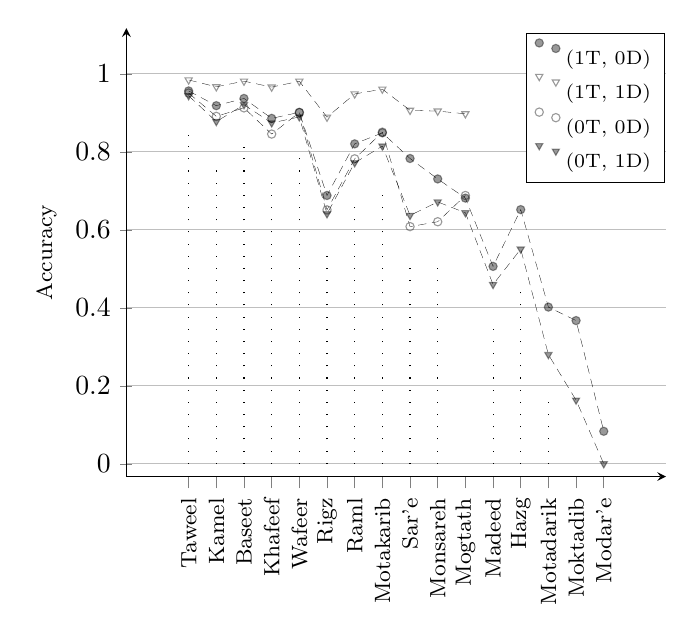
\begin{tikzpicture}[scale=1]
  \begin{axis}[
    axis x line = bottom,
    axis y line = left,
    ymajorgrids = true,
    ybar,
    enlargelimits=0.15,
    legend style={at={(0.87,0.99)},
      anchor=north,legend columns=1},
    ylabel={Accuracy},
    ylabel style = {font=\footnotesize},
    symbolic x coords={Taweel, Kamel, Baseet, Khafeef, Wafeer, Rigz, Raml, Motakarib, Sar'e, Monsareh, Mogtath, Madeed, Hazg, Motadarik, Moktadib, Modar'e},
    xtick=data,
    xticklabel style = {font=\footnotesize},
    nodes near coords align={vertical},
    x tick label style={rotate=90, anchor=east},
    bar width=2pt,
    ymin=0.1,
    ]


	
	% full diacritic (Full Circle)
	% replaced
	% Exp_3_full_data_matrix_with_tashkeel_8bitsEncoding_Bidirectional_LSTM_3_82_0
	% (0T, 1D)
	\addplot[mark=*, thin, only marks, mark size=1.5pt, point
	meta=explicit symbolic, opacity=0.4]
	coordinates {
		(Wafeer,    0.9014024346835623 )       
		(Monsareh,  0.7305790960451978 )       
		(Madeed,    0.5062814070351759 )  
		(Mogtath,   0.6814562002275313 )       
		(Motakarib, 0.8488725411802335 )       
		(Kamel,     0.9185383195083638 )       
		(Taweel,    0.9563337122522612 )       
		(Sar'e,     0.7830334190231363 )       
		(Raml,      0.8205778003041054 )       
		(Rigz,      0.6881982360352793 )       
		(Khafeef,   0.8859834647183235 )       
		(Baseet,    0.9370664229634861 ) 
		(Moktadib,  0.3673469387755102 ) 
		(Hazg,      0.6519480519480519 )
		(Modar'e,   0.08333333333333333)
		(Motadarik, 0.40190476190476193) 
	};


    % trimmed no-diacritic (Empty Triangle)
    \addplot[mark=triangle, every mark/.append style={rotate=180},
    thin, only marks, mark size=1.5pt, point meta=explicit symbolic, opacity=0.4]
    coordinates {
      % replaced
      % Exp_3_eliminated_data_matrix_without_tashkeel_8bitsEncoding_Bidirectional_LSTM_3_82_0
      % (1T, 0D)
      (Wafeer,    0.9811213222198475)       
      (Monsareh,  0.9045746962115797)       
      (Mogtath,   0.897708216880939 )       
      (Motakarib, 0.9609120521172638)       
      (Kamel,     0.966898378020523 )       
      (Taweel,    0.9844991757498216)       
      (Sar'e,     0.9066397034041119)       
      (Raml,      0.9485771342985522)       
      (Rigz,      0.8889925373134329)       
      (Khafeef,   0.9661488673139158)       
      (Baseet,    0.9814341393906374) 
      % Damn Trick; the first \addplot must have all the x ticks; otherwise
      % the following 4 ticks will not appear on the x-axis.
      %(Madeed,     0)  
      %(Hazg,       0) 
      %(Motadarik,  0) 
      %(Moktadib,   0) 
      %(Modar'e,    0)
    };

    % trimmed diacritic (Empty Circle)
    % replaced
    % Exp_3_eliminated_data_matrix_with_tashkeel_8bitsEncoding_Bidirectional_LSTM_3_82_0 
    % (1T, 1D)
    \addplot[mark=o, thin, only marks, mark size=1.5pt, point
    meta=explicit symbolic, opacity=0.4]
    coordinates{
      (Wafeer,     0.9009759920210871)       
      (Monsareh,   0.6208005718370264)       
      (Mogtath,    0.6880939072107323)       
      (Motakarib,  0.8506281991624011)       
      (Kamel,      0.8910956636875207)       
      (Taweel,     0.9508402430922914)       
      (Sar'e,      0.6083586113919784)       
      (Raml,       0.7822016974538193)       
      (Rigz,       0.6512042062415196)       
      (Khafeef,    0.8456957928802589)       
      (Baseet,     0.9128703742508696) 
    };


    % full no-diacritic (Full Triangle)
    % replaced
    % Exp_3_full_data_matrix_without_tashkeel_8bitsEncoding_Bidirectional_LSTM_3_82_0
    % (0T, 0D)
    \addplot[mark=triangle*, every mark/.append style={rotate=180},
    thin, only marks, mark size=1.5pt, point meta=explicit symbolic, opacity=0.4]
    coordinates {
      (Wafeer,    0.889584964761159  )       
      (Monsareh,  0.6716101694915254 )       
      (Madeed,    0.45979899497487436)  
      (Mogtath,   0.6439135381114903 )       
      (Motakarib, 0.8148088917319687 )       
      (Kamel,     0.8776972469479428 )       
      (Taweel,    0.9439529481540059 )       
      (Sar'e,     0.6370179948586119 )       
      (Raml,      0.7719209325899645 )       
      (Rigz,      0.64107517849643   )       
      (Khafeef,   0.8741908607319105 )       
      (Baseet,    0.9208657001620072 ) 
      (Moktadib,  0.16326530612244897) 
      (Hazg,      0.5506493506493506 )
      (Modar'e,   0.0                )
      (Motadarik, 0.28               ) 
    };

    \legend{
      {\scriptsize (1T, 0D)},
      {\scriptsize (1T, 1D)},
      {\scriptsize (0T, 0D)},
      {\scriptsize (0T, 1D)},
    }

    % Dotted line
    \draw[loosely dotted] (axis cs:Wafeer,    0) -- (axis cs:Wafeer,     0.789584964761159);
    \draw[loosely dotted] (axis cs:Monsareh,  0) -- (axis cs:Monsareh,   0.5208005718370264);
    \draw[loosely dotted] (axis cs:Mogtath,   0) -- (axis cs:Mogtath,    0);
    \draw[loosely dotted] (axis cs:Motakarib, 0) -- (axis cs:Motakarib,  0.7148088917319687);
    \draw[loosely dotted] (axis cs:Kamel,     0) -- (axis cs:Kamel,      0.7776972469479428);
    \draw[loosely dotted] (axis cs:Taweel,    0) -- (axis cs:Taweel,     0.8439529481540059);
    \draw[loosely dotted] (axis cs:Sar'e,     0) -- (axis cs:Sar'e,      0.5083586113919784);
    \draw[loosely dotted] (axis cs:Raml,      0) -- (axis cs:Raml,       0.6719209325899645);
    \draw[loosely dotted] (axis cs:Rigz,      0) -- (axis cs:Rigz,       0.54107517849643);
    \draw[loosely dotted] (axis cs:Khafeef,   0) -- (axis cs:Khafeef,    0.7456957928802589);
    \draw[loosely dotted] (axis cs:Baseet,    0) -- (axis cs:Baseet,     0.8128703742508696);
    \draw[loosely dotted] (axis cs:Moktadib,  0) -- (axis cs:Moktadib,   0);
    \draw[loosely dotted] (axis cs:Madeed,    0) -- (axis cs:Madeed,     0.35979899497487436);
    \draw[loosely dotted] (axis cs:Hazg,      0) -- (axis cs:Hazg,       0.4506493506493506);
    \draw[loosely dotted] (axis cs:Modar'e,   0) -- (axis cs:Modar'e,    0);
    \draw[loosely dotted] (axis cs:Motadarik, 0) -- (axis cs:Motadarik,  0.18);


    % connecting a models accuracies

    % Empty Triangle
    % (1T, 0D)
    \draw[line width=0.1pt, densely dashed]
    (axis cs:Taweel,        0.9844991757498216)
    -- (axis cs:Kamel,      0.966898378020523 )
    -- (axis cs:Baseet,     0.9814341393906374)
    -- (axis cs:Khafeef,    0.9661488673139158)
    -- (axis cs:Wafeer,     0.9811213222198475)
    -- (axis cs:Rigz,       0.8889925373134329)
    -- (axis cs:Raml,       0.9485771342985522)
    -- (axis cs:Motakarib,  0.9609120521172638)
    -- (axis cs:Sar'e,      0.9066397034041119)
    -- (axis cs:Monsareh,   0.9045746962115797)
    -- (axis cs:Mogtath,    0.897708216880939 );

   % Empty Circle
   % (1T, 1D)
   \draw[line width=0.1pt, densely dashed]
   (axis cs:Taweel,        0.9508402430922914)
   -- (axis cs:Kamel,      0.8910956636875207)
   -- (axis cs:Baseet,     0.9128703742508696)
   -- (axis cs:Khafeef,    0.8456957928802589)
   -- (axis cs:Wafeer,     0.9009759920210871)
   -- (axis cs:Rigz,       0.6512042062415196)
   -- (axis cs:Raml,       0.7822016974538193)
   -- (axis cs:Motakarib,  0.8506281991624011)
   -- (axis cs:Sar'e,      0.6083586113919784)
   -- (axis cs:Monsareh,   0.6208005718370264)
   -- (axis cs:Mogtath,    0.6880939072107323);


    % Full Triangle
    % (0T, 0D)
    \draw[line width=0.1pt, densely dashed]
    (axis cs:Taweel,        0.9439529481540059 )
    -- (axis cs:Kamel,      0.8776972469479428 )
    -- (axis cs:Baseet,     0.9208657001620072 )
    -- (axis cs:Khafeef,    0.8741908607319105 )
    -- (axis cs:Wafeer,     0.889584964761159  )
    -- (axis cs:Rigz,       0.64107517849643   )
    -- (axis cs:Raml,       0.7719209325899645 )
    -- (axis cs:Motakarib,  0.8148088917319687 )
    -- (axis cs:Sar'e,      0.6370179948586119 )
    -- (axis cs:Monsareh,   0.6716101694915254 )
    -- (axis cs:Mogtath,    0.6439135381114903 )
    -- (axis cs:Madeed,     0.45979899497487436)
    -- (axis cs:Hazg,       0.5506493506493506 )
    -- (axis cs:Motadarik,  0.28               )
    -- (axis cs:Moktadib,   0.16326530612244897)
    -- (axis cs:Modar'e,    0.0                );


   % Full Circle
   % (0T, 1D)
   \draw[line width=0.1pt, densely dashed]
   (axis cs:Taweel,        0.9563337122522612 )
   -- (axis cs:Kamel,      0.9185383195083638 )
   -- (axis cs:Baseet,     0.9370664229634861 )
   -- (axis cs:Khafeef,    0.8859834647183235 )
   -- (axis cs:Wafeer,     0.9014024346835623 )
   -- (axis cs:Rigz,       0.6881982360352793 )
   -- (axis cs:Raml,       0.8205778003041054 )
   -- (axis cs:Motakarib,  0.8488725411802335 )
   -- (axis cs:Sar'e,      0.7830334190231363 )
   -- (axis cs:Monsareh,   0.7305790960451978 )
   -- (axis cs:Mogtath,    0.6814562002275313 )
   -- (axis cs:Madeed,     0.5062814070351759 )
   -- (axis cs:Hazg,       0.6519480519480519 )
   -- (axis cs:Motadarik,  0.40190476190476193)
   -- (axis cs:Moktadib,   0.3673469387755102 )
   -- (axis cs:Modar'e,    0.08333333333333333);

  \end{axis}
\end{tikzpicture}


%%% Local Variables:
%%% mode: latex
%%% TeX-master: "../../master"
%%% End:
	\caption{The per-class accuracy score of the best four models.}~\label{Fig:ArabicModelsResults}
\end{figure}
}

\end{frame}
%%%%%%%%%%%%%%%%%%%%%%%%%%%%%%%%%%%%%%%%%%%%%%%%%%

\section{Discussions}


%%%%%%%%%%%%%%%%%%%%%%%%%%%%%%%%%%%%%%%%%%%%%%%%%%
\begin{frame}[fragile]{Encoding effect}
%\Wider{
	\begin{figure}[!t]
		  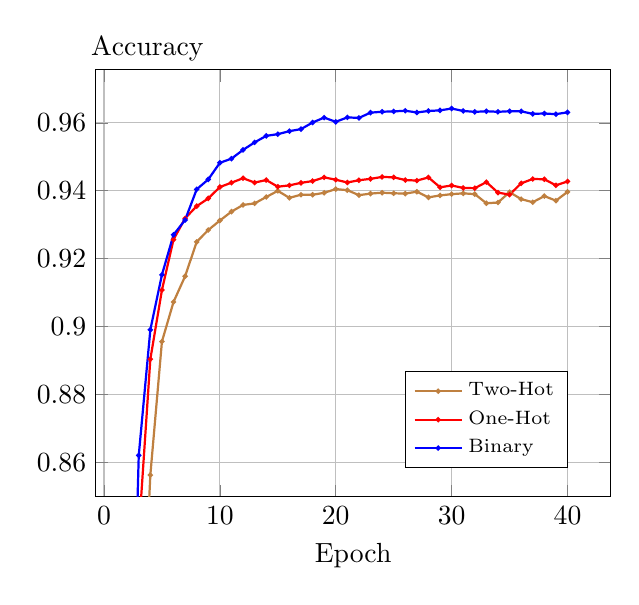
\begin{tikzpicture}
		\begin{axis}[
  height=7cm,
  grid=major,
  every axis y label/.style= {at={( 0.1, 1.1)}, anchor=north},
  xlabel={Epoch},
  ylabel={Accuracy},
  % every axis y label/.style= {at={( 0.1, 1.1)}, anchor=north},
  legend style={at={(0.6, 0.18)},anchor=west},
  % legend style={at={(0.5, -0.30)}, anchor=north, legend columns=3},
  every axis legend/.append style={nodes={right}},
  ymin = 0.85,
  name=left plot,
  title style={at={(0.5,-.4)}}
  ]



  \addplot[color=brown, mark=*, thick, mark size=0.5pt] coordinates {

    % twohot
    (1,      0.4973408579826355 )
    (2,      0.6637325882911682 )
    (3,      0.7843776345252991 )
    (4,      0.8562803268432617 )
    (5,      0.8955804109573364 )
    (6,      0.9072529673576355 )
    (7,      0.9148279428482056 )
    (8,      0.9249432682991028 )
    (9,      0.9284470081329346 )
    (10,     0.9312249422073364 )
    (11,     0.9338576793670654 )
    (12,     0.9358240365982056 )
    (13,     0.9362859129905701 )
    (14,     0.9381598234176636 )
    (15,     0.9399744272232056 )
    (16,     0.9379156827926636 )
    (17,     0.9388328790664673 )
    (18,     0.9388262629508972 )
    (19,     0.939400315284729 )
    (20,     0.9404956698417664 )
    (21,     0.9401789307594299 )
    (22,     0.9387009143829346 )
    (23,     0.9391694068908691 )
    (24,     0.9394267201423645 )
    (25,     0.939261794090271 )
    (26,     0.9391694068908691 )
    (27,     0.9397236704826355 )
    (28,     0.9380608797073364 )
    (29,     0.9386216998100281 )
    (30,     0.9390044212341309 )
    (31,  0.9392420053482056)
    (32,  0.9390110373497009)
    (33,  0.9363254904747009)
    (34,  0.9365366101264954)
    (35,  0.9395982623100281)
    (36,  0.9375395774841309)
    (37,  0.9366289973258972)
    (38,  0.9384303689002991)
    (39,  0.9370908737182617)
    (40,  0.9396642446517944)
  };
  % \addlegendentry{Two-Hot}





  \addplot[color=red, mark=*, thick, mark size=0.5pt] coordinates {
    % onehot
    (1,        0.5241501331329346 )
    (2,        0.6912611126899719 )
    (3,        0.8391179442405701 )
    (4,        0.8904072642326355 )
    (5,        0.9107500910758972 )
    (6,        0.9256294965744019 )
    (7,        0.9318781495094299 )
    (8,        0.9354742765426636 )
    (9,        0.9377507567405701 )
    (10,       0.9410961270332336 )
    (11,       0.9423761963844299 )
    (12,       0.9436959028244019 )
    (13,       0.9424092173576355 )
    (14,       0.9431548118591309 )
    (15,       0.9411951303482056 )
    (16,       0.9415910243988037 )
    (17,       0.942330002784729 )
    (18,       0.9428513050079346 )
    (19,       0.9439400434494019 )
    (20,       0.9432538151741028 )
    (21,       0.9424421787261963 )
    (22,       0.9430954456329346 )
    (23,       0.9435111284255981 )
    (24,       0.9440720081329346 )
    (25,       0.9439598321914673 )
    (26,       0.9431614279747009 )
    (27,       0.9429964423179626 )
    (28,       0.9439268112182617 )
    (29,       0.9410235285758972 )
    (30,       0.9415580034255981 )
    (31,  0.9408321976661682)
    (32,  0.9407595992088318)
    (33,  0.9425477981567383)
    (34,  0.939453125 )
    (35,  0.9388592839241028)
    (36,  0.942191481590271 )
    (37,  0.9434715509414673)
    (38,  0.9433857798576355)
    (39,  0.9416041970252991)
    (40,  0.9427457451820374)
  };
  % \addlegendentry{One-Hot}




  \addplot[color=blue, mark=*, thick, mark size=0.5pt] coordinates {
    % binary
    (1,         0.4176618158817291)
    (2,         0.7385522127151489)
    (3,         0.8620811104774475)
    (4,         0.8990639448165894)
    (5,         0.9152568578720093)
    (6,         0.9270322322845459)
    (7,         0.9314031600952148)
    (8,         0.9404243230819702)
    (9,         0.9433448910713196)
    (10,        0.9482346773147583)
    (11,        0.9494454860687256)
    (12,        0.9520400762557983)
    (13,        0.9542421698570251)
    (14,        0.956171452999115 )
    (15,        0.9566637873649597)
    (16,        0.9575485587120056)
    (17,        0.9581539630889893)
    (18,        0.9601032733917236)
    (19,        0.9615402817726135)
    (20,        0.9603028297424316)
    (21,        0.9616068005561829)
    (22,        0.9614471197128296)
    (23,        0.9629971981048584)
    (24,        0.9632699489593506)
    (25,        0.9633697867393494)
    (26,        0.9635560512542725)
    (27,        0.9630637168884277)
    (28,        0.9634895324707031)
    (29,        0.9636757969856262)
    (30,        0.9642080068588257)
    (31, 0.963502824306488 )
    (32, 0.9632300734519958)
    (33, 0.9634096622467041)
    (34, 0.9632500410079956)
    (35, 0.963416337966919 )
    (36, 0.9633830785751343)
    (37, 0.962651252746582 )
    (38, 0.962751030921936 )
    (39, 0.9625581502914429)
    (40, 0.9630969762802124)
  };
  % \addlegendentry{Binary}



  \legend{
    {\scriptsize Two-Hot},
    {\scriptsize One-Hot},
    {\scriptsize Binary},
  }

  % \legend{Binary\hspace*{8pt}, One-Hot\hspace*{8pt}, Two-Hot}
\end{axis}


%%% Local Variables:
%%% mode: latex
%%% TeX-master: "../../master"
%%% End:
		  \end{tikzpicture}
		\caption{Encoding effect on Learning rate with the best model (1T, 0D, 4L, 82U, 0W, BinE) and when using the two other encodings	instead of BinE.}~\label{Fig:ArabicModelsResults}

	\end{figure}
%}

\end{frame}

%%%%%%%%%%%%%%%%%%%%%%%%%%%%%%%%%%%%%%%%%%%%%%%%%%


\begin{frame}[fragile]{Encoding effect}

\begin{block}{Encoding}
	\begin{itemize}
		
		\item The encoding method is a transformer function $\mathcal{T}$ which transform a discrete input values $X$. 
		\item If the network $\eta_1$ is the most accurate network which can ``decode'' $\mathcal{T}(X)$. 
		\item If we have another encoding function $\mathcal{T}_2$ and we tried to use the same network $\eta_1$ for the $\mathcal{T}_2$ as $\eta_1\left(\mathcal{T}_1(X)\right) = \left(\eta_1\cdot\mathcal{T}_1\cdot \mathcal{T}_2^{-1} \right)\left(\mathcal{T}_2(X)\right)$. This network may be of complicated architecture to be able to “decode” a terse or complex pattern $\mathcal{T}_2(X)$.
		
		
	\end{itemize}

	
\end{block}

\end{frame}

%%%%%%%%%%%%%%%%%%%%%%%%%%%%%%%%%%%%%%%%%%%%%%%%%%
\begin{frame}[fragile]{Classifying Arabic Non-Poem Text}
\begin{Arabic}
	\begin{traditionalpoem}
		خلال المباراة التي جمعتهما\quad & \quad  مساء السبت بالجولة الـ26 من المسابقة \\
		%خِلَالَ الْمُبَارَاةِ الْلَتِي جَمْعَتِهِمَا\quad & \quad مَسَاءَ السْسَبْتِ بِالْجَوْلَةِ ال26 مِنَ الْمُسَابَقَةِ \\
		{\color{purple} خلالَلْ} {\color{blue} مُباراتل} {\color{OliveGreen} لَتِيجُ} {\color{Brown} مَعَتْهُما}\quad & \quad
		{\color{purple} مِساءَسْ} {\color{blue} سَبَتْبِلْجَوْ} {\color{OliveGreen} لَتِلْمِنَلْ } {\color{Brown} مُسَابَقَه}\\
		
		{\color{purple} \texttt{0/0//}} {\color{blue} \texttt{0/0/0//}} {\color{OliveGreen} \texttt{/0//}} {\color{Brown} \texttt{0//0//}}\quad & \quad
		{\color{purple} \texttt{0/0//}} {\color{blue} \texttt{0/0/0//}}  \texttt{{\color{OliveGreen}/0//}{\color{red}/}{\color{OliveGreen}0}} {\color{Brown} \texttt{0//0//}}\\
		{\color{purple} \texttt{0/0//}} {\color{blue} \texttt{0/0/0// }} {\color{OliveGreen} \texttt{/0//}} {\color{Brown} \texttt{0/0///}}\quad & \quad
		{\color{purple} \texttt{0/0//}} {\color{blue} \texttt{0/0/0//}} {\color{OliveGreen} \texttt{0/0//}} {\color{Brown} \texttt{0//0//}}\\
		
		{\color{purple} فَعُوْلُنْ} {\color{blue} مَفَاعِيْلُنْ} {\color{OliveGreen} فَعُولُ} {\color{Brown} مَفَاعِلُنْ}\quad & \quad
		{\color{purple} فَعُوْلُنْ} {\color{blue} مَفَاعِيْلُنْ} {\color{OliveGreen} فَعُوْلُنْ} {\color{Brown} مَفَاعِيْلُنْ}
		
	\end{traditionalpoem}
\end{Arabic}

\end{frame}

%%%%%%%%%%%%%%%%%%%%%%%%%%%%%%%%%%%%%%%%%%%%%%%%%%


%%%%%%%%%%%%%%%%%%%%%%%%%%%%%%%%%%%%%%%%%%%%%%%%%%
\begin{frame}[fragile]{Classifying Arabic Non-Poem Text}
\begin{figure}[!t]
{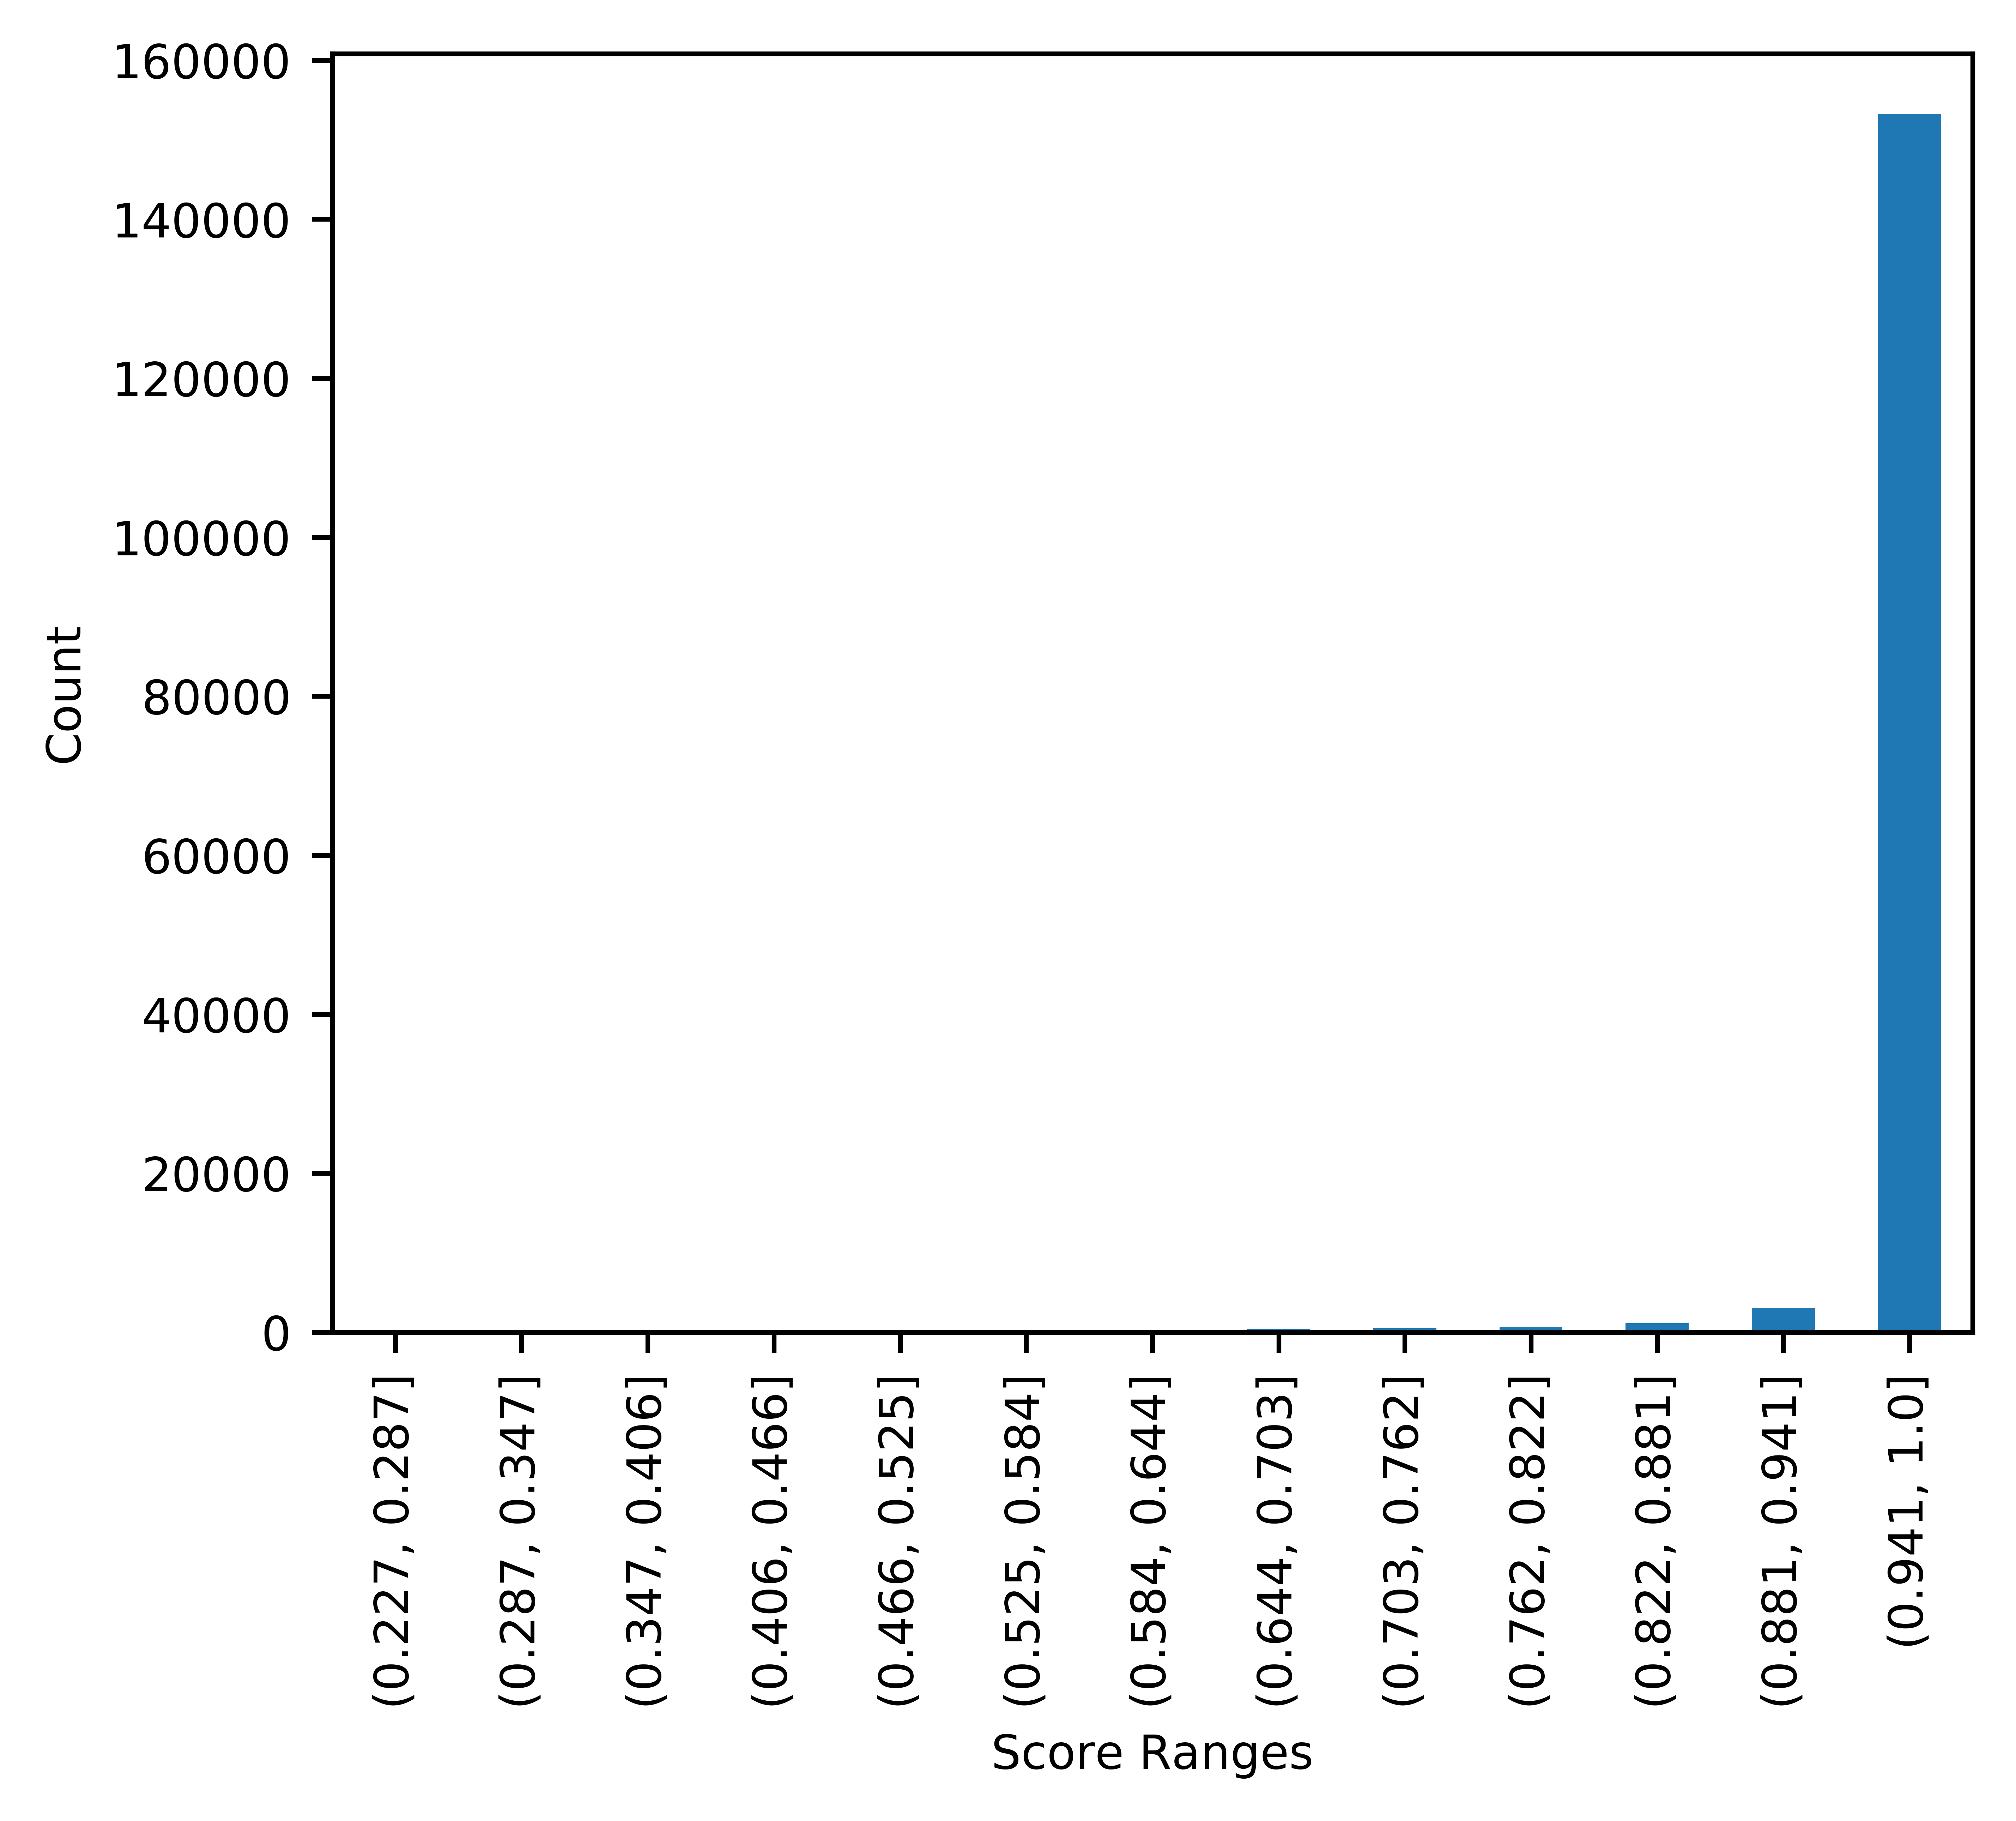
\includegraphics[scale=.65]{./Figures/IMG_Result_Distribution.png}};
	\caption{Testing data score ranges distribution.}
\end{figure}

\end{frame}

%%%%%%%%%%%%%%%%%%%%%%%%%%%%%%%%%%%%%%%%%%%%%%%%%%
\begin{frame}

\begin{thebibliography}{10}
	
	\bibitem{Abuata2016RuleBasedAlgorithm}
	\alert{Abuata, Belal and Al-Omari, Asma}
	\newblock  {A Rule-Based Algorithm for the Detection of Arud Meter in Classical Arabic Poetry}
	\newblock {\em International Arab Journal of Information Technology. (2017), 15}.
	
	\bibitem{Alnagdawi2013FindingArabicPoemMeter}
	\alert{Alnagdawi, Mohammad and Rashaideh, Hasan and Aburumman, Ala}
	\newblock  {Finding Arabic Poem Meter Using Context Free Grammar}
	\newblock {\em J. of Commun. {\&} Comput. Eng. (2013), 3, 52-59}.
	
	\bibitem{colah}
	\alert{Colah}
	\newblock  {Understanding Lstm Networks}
	\newblock {\em http://colah.github.io/posts/2015-08-Understanding-LSTMs/ , 2015}.
	
	\bibitem{Gitrepo_NN_Tikz}
	\alert{Petar Veličković}
	\newblock  {Collection of Latex Tikz figures}
	\newblock {\em https://github.com/PetarV-/TikZ}.
%	
%	\bibitem{al-farahidi}
%	\alert{Ibrahim Osman}
%	\newblock {\em https://goo.gl/ZJySa8}.
	
	
	
\end{thebibliography}
\end{frame}


%%%%%%%%%%%%%%%%%%%%%%%%%%%%%%%%%%%%%%%%%%%%%%%%%%%%%%%%%%%%%%%%%%%%%%%%%%%


%%%%%%%%%%%%%%%%%%%%%%%%%%%%%%%%%%%%%%%%%%%%%%%%%%
\begin{frame}[fragile]{Questions!}
\begin{center}
	Questions.
\end{center}

\end{frame}

%%% Local Variables:
%%% mode: latex
%%% TeX-master: "../main"
%%% TeX-engine: xetex
%%% End:
